\documentclass[11pt,a5paper,twoside,bahasa,listof=nochaptergap]{book}
\usepackage[tmargin=2.5cm,bmargin=2.5cm,lmargin=2.5cm,rmargin=2.0cm]{geometry}
\setcounter{secnumdepth}{5}
\setcounter{tocdepth}{5}
\usepackage[titletoc]{appendix}
\usepackage{csvsimple,longtable,booktabs}
\usepackage{listings}
\usepackage{diagbox}
\usepackage{csquotes}
\usepackage{tikz}
\usetikzlibrary{shapes.geometric,arrows,fit,matrix,positioning,shadows,graphs}


%\usetikzlibrary{graphs,graphdrawing,arrows.meta,external}

\tikzset
{
    treenode/.style = {circle, draw=black, align=center, minimum size=1cm},
    splitnode/.style = {circle, draw=black, align=center, minimum size=1cm, fill=black!30!white},
    subtree/.style  = {isosceles triangle, draw=black, align=center, minimum height=0.5cm, minimum width=1cm, shape border rotate=90, anchor=north}
    missing/ 
}

\usepackage{amsmath}
\usepackage[titles]{tocloft}

\begingroup
\makeatletter
\let\newcounter\@gobble\let\setcounter\@gobbletwo
\globaldefs\@ne \let\c@loldepth\@ne
\newlistof{listings}{lol}{\lstlistlistingname}
\newlistentry{lstlisting}{lol}{0}
\makeatother
\endgroup

\cftsetindents{lstlisting}{0in}{1.3in}

\lstset{ %
	language = C++,
	numbers=left,
	xleftmargin=2em,
	xrightmargin=2mm,
	frame=single,
	framesep=2mm,
	basicstyle=\footnotesize\ttfamily,
	framexleftmargin=2em,
	captionpos=b,
	belowcaptionskip=4pt,
	frame=single,
	breaklines=true,
	postbreak=\raisebox{0ex}[0ex][0ex]{\ensuremath{\color{red}\hookrightarrow\space}}
}
\usepackage{color, colortbl}
\definecolor{LightCyan}{rgb}{0.88,1,1}
\usepackage{rotating}
\usepackage{mdframed}
\usepackage{clrscode3e}
\usepackage[parfill]{parskip}
\usepackage{graphics}
\usepackage{fontspec}
\usepackage{subcaption}
\setsansfont{Trebuchet MS}
\setmainfont{Times New Roman}
\setmonofont{Courier New}
\usepackage{tocbibind}
\usepackage{enumitem}
\usepackage{pdflscape}
\usepackage{minted}
\usepackage{multirow}
\usepackage[verbose]{wrapfig}
\usepackage{changepage}
\usepackage{eso-pic}
\usepackage{ragged2e}
\usepackage{xesearch}
\usepackage[bahasa]{babel}
\usepackage[breaklinks=true]{hyperref}
\usepackage[font=small]{caption}
\usepackage{enumitem}
\setlist{nolistsep}
\usepackage{float}
\usepackage{longtable}
\usepackage{array,etoolbox}
\usepackage{amssymb}
\preto\tabular{\setcounter{magicrownumbers}{0}}
\preto\longtable{\setcounter{magicrownumbers}{0}}
\newcounter{magicrownumbers}
\newcommand\rownumber{\stepcounter{magicrownumbers}\arabic{magicrownumbers}}

\newcommand\nc[1]{%
	\multicolumn{1}{c}{#1}%
}

\usepackage{setspace}
\singlespacing
\usepackage{fancyhdr}
\fancyhf{}
\renewcommand{\headrulewidth}{0pt}
\lhead[\thepage]{}
\rhead[]{\thepage}
\pagestyle{fancy}

\usepackage{titlesec}
\titleformat{\chapter}[display]{\filcenter\fontsize{11}{11}\bfseries}{\chaptername \ \thechapter}{0pt}{\filcenter\fontsize{11}{11}\bfseries\uppercase}
\titlespacing*{\chapter}{0pt}{-0.5cm}{40pt}
\titlespacing*{\section}{0pt}{11pt}{0pt}
\titlespacing*{\subsection}{0pt}{11pt}{0pt}
\titlespacing*{\subsubsection}{0pt}{11pt}{0pt}
\titleformat*{\section}{\fontsize{11}{11}\bfseries}
\titleformat*{\subsection}{\fontsize{11}{11}\bfseries}
\titleformat*{\subsubsection}{\fontsize{11}{11}\bfseries}


\addto\captionsbahasa{%
	\renewcommand\bibname{DAFTAR PUSTAKA}%
	\renewcommand\contentsname{DAFTAR ISI}%
	\renewcommand\listtablename{DAFTAR TABEL}%
	\renewcommand\listfigurename{DAFTAR GAMBAR}%
	\renewcommand\chaptername{BAB}%
}


\usepackage{chngcntr}
\renewcommand{\lstlistingname}{Kode Sumber}
\renewcommand{\lstlistlistingname}{DAFTAR KODE SUMBER}
\renewcommand*\thechapter{\arabic{chapter}}
\renewcommand\cftlstlistingpresnum{Kode Sumber }
\newcommand{\var}[2]{\newcommand{#1}{#2}}
\var{\judul}{Penerapan Konsep DSU on Tree dan Struktur Data Segment Tree Pada Rancang Algoritma: Studi Kasus SPOJ Klasik LIS and TREE}
\var{\judulEnglish}{Implementation of DSU on Tree Concept and Segmnt Tree Data Structure on Algorithm Design on: Case Study in SPOJ Classic Problem LIS and TREEE}
\var{\gelar}{Sarjana Komputer}
\var{\penulis}{Dimas Hirda Pratama}
\var{\nrp}{05111440000147}
\var{\jurusan}{Informatika }
\var{\jurusanEnglish}{Informatics Department }
\var{\fakultas}{Teknologi Informasi dan Komunikasi}
\var{\fakultasEnglish}{Information Technology and Communication}
\var{\prodi}{S-1 }
\var{\bidangStudi}{Algoritma Pemrograman}
\var{\pembimbingSatu}{Rully Soelaiman, S.Kom., M.Kom.}
\var{\nipPembimbingSatu}{197002131994021001}
\var{\pembimbingDua}{Abdul Munif, S.Kom., M.Sc.}
\var{\nipPembimbingDua}{198608232015041004}
\var{\problem}{permasalahan klasik \textit{LIS and TREE}}
\var{\tahun}{2018}


\usepackage{caption}
\captionsetup[table]{labelsep=space}
\captionsetup[figure]{labelsep=space}
\captionsetup[lstlisting]{labelsep=space}

\setlength\cftparskip{-2pt}
\setlength\cftbeforechapskip{0pt}
\setlength{\lineskip}{0pt}

% Pemenggalan Tambahan
%english
%\hyphenation{ver-tex}
%\hyphenation{bridge}
%\hyphenation{block}
%\hyphenation{weight}
%\hyphenation{dis-joint}
%\hyphenation{par-ent}
%\hyphenation{root}
%\hyphenation{node}
%\hyphenation{set}
%\hyphenation{bridge-block}
%\hyphenation{con-nected}
%\hyphenation{com-po-nent}
%\hyphenation{undi-rected}
%\hyphenation{di-rected}
%\hyphenation{par-tially}
%\hyphenation{fully}
%\hyphenation{query}
%\hyphenation{dataset}

%bahasa
\hyphenation{me-nge-ta-hui}
\hyphenation{me-nya-ta-kan}
\hyphenation{meng-i-ni-si-al-i-sa-si}
\hyphenation{meng-gu-na-kan}
\hyphenation{me-la-ku-kan}
\hyphenation{me-li-bat-kan}
\hyphenation{per-ma-sa-la-han}
\hyphenation{struk-tur}

\makeatletter
\def\emptypage@emptypage{%
	\begin{center}
		\emph{Halaman ini sengaja dikosongkan}
	\end{center}
	\newpage%
}%
\def\cleardoublepage{%
	\clearpage%
	\if@twoside%
	\ifodd\c@page%
	% do nothing
	\else%
	\emptypage@emptypage%
	\fi%
	\fi%
}%
\makeatother
\raggedbottom


\renewcommand{\cftchapleader}{\cftdotfill{\cftdotsep}}
\renewcommand{\cftchappresnum}{BAB }
\renewcommand{\cfttabpresnum}{Tabel }
\cftsetindents{tab}{1em}{4.7em}
\renewcommand{\cftfigpresnum}{Gambar }
\cftsetindents{fig}{1em}{5.5em}

\cftsetindents{chapter}{0em}{3.6em}      % set amount of 
\cftsetindents{section}{2em}{2em}

\renewcommand{\thechapter}{\Roman{chapter}}
\renewcommand{\thesection}{\arabic{chapter}.\arabic{section}}
\renewcommand{\thesubsection}{\arabic{chapter}.\arabic{section}.\arabic{subsection}}
\renewcommand{\thefigure}{\arabic{chapter}.\arabic{figure}}
\renewcommand{\thetable}{\arabic{chapter}.\arabic{table}}

\newcommand{\insertfigure}{\begin{figure}\caption{A figure}\end{figure}}
\usepackage{etoolbox}% http://ctan.org/pkg/etoolbox
\makeatletter
% \patchcmd{<cmd>}{<search>}{<replace>}{<succes>}{<failure>}
\patchcmd{\@chapter}{\addtocontents{lof}{\protect\addvspace{10\p@}}}{}{}{}
\patchcmd{\@chapter}{\addtocontents{lot}{\protect\addvspace{10\p@}}}{}{}{}
\makeatother

\makeatletter
\g@addto@macro\appendix{%
	\addtocontents{toc}{%
		\protect\renewcommand{\protect\cftchappresnum}{}%
	}%
}
\makeatother


\renewcommand{\cftchapaftersnumb}{\hspace{0em}}

% Table caption above table
\floatstyle{plaintop}
\restylefloat{table}

% Centering table caption
\usepackage[justification=centering]{caption}
% Prevent hyphenation
\usepackage[none]{hyphenat}

\usepackage{mfirstuc}
\newcommand\addvmargin[1]{
	\node[fit=(current bounding box),inner ysep=#1,inner xsep=0]{};
}

\usepackage{tikz}
\usepackage[normalem]{ulem}

\begin{document} \sloppy
	% To prevent lstlisting from roman numbering
	\renewcommand{\thelstlisting}{\arabic{chapter}.\arabic{lstlisting}}
	\renewcommand{\theequation}{\arabic{chapter}.\arabic{equation}}
	
	% To remove spacing between chapter in list of figure and list of table
	\addtocontents{lof}{\protect\renewcommand*\protect\addvspace[1]{}}
	\addtocontents{lot}{\protect\renewcommand*\protect\addvspace[1]{}}
	
	% \setlength{\abovecaptionskip}{-12.75pt}
	
	\title {\judul}
	\author {\penulis}
	
	\frontmatter
	\addcontentsline{toc}{chapter}{SAMPUL}
	\newpage
	\newgeometry{top=7cm,left=2cm,bottom=2cm}

	\sffamily
	\thispagestyle{empty}
	\color{white}
	{ \noindent TUGAS AKHIR - KI141502 }\\*[10pt] 
	{\large\textbf{\MakeUppercase{\judul}}} \\*[32pt]
	\\
	\\
	\\
	\MakeUppercase{\penulis} \\*
	NRP \nrp \\*[10pt]
	Dosen Pembimbing 1 \\*
	\pembimbingSatu \\*[10pt]
	Dosen Pembimbing 2 \\*
	\pembimbingDua \\*[10pt]
	DEPARTEMEN \MakeUppercase{\jurusan} \\*
	Fakultas \fakultas \\*
	Institut Teknologi Sepuluh Nopember \\*
	Surabaya, \tahun \\*
	\AddToShipoutPictureBG*{
\includegraphics[width=\paperwidth,height=\paperheight]{sampul/sampul.png}}
	\rmfamily
	\normalsize
	\restoregeometry
	\color{black}
	\cleardoublepage
	
\newpage
	\newgeometry{top=7cm,left=2cm,bottom=2cm}

	\sffamily
	\thispagestyle{empty}
	{ \noindent TUGAS AKHIR - KI141502 }\\*[10pt] 
	{\large\textbf{\MakeUppercase{\judul}}} \\*[32pt]
	\\
	\\
	\\
	\MakeUppercase{\penulis} \\*
	NRP \nrp \\*[10pt]
	Dosen Pembimbing 1 \\*
	\pembimbingSatu \\*[10pt]
	Dosen Pembimbing 2 \\*
	\pembimbingDua \\*[10pt]
	DEPARTEMEN \MakeUppercase{\jurusan} \\*
	Fakultas \fakultas \\*
	Institut Teknologi Sepuluh Nopember \\*
	Surabaya, \tahun \\*
	\AddToShipoutPictureBG*{
\includegraphics[width=\paperwidth,height=\paperheight]{sampul/sampulWhite.png}}
	\rmfamily
	\normalsize
	\restoregeometry
	\color{black}
	\cleardoublepage

\newpage
	\newgeometry{top=7cm,left=2cm,bottom=2cm}
	\sffamily
	\thispagestyle{empty}
	{\noindent UNDERGRADUATE THESES - KI141502 } \\*[10pt]
	{\large\textbf{\MakeUppercase{\judulEnglish}}} \\*[32pt]
	\\
	\\
	\\
	\\
	\MakeUppercase{\penulis} \\*
	NRP \nrp \\*[10pt]
	Supervisor 1 \\*
	\pembimbingSatu \\*[10pt]
	Supervisor 2 \\*
	\pembimbingDua \\*[10pt]
	\MakeUppercase{\jurusanEnglish} \\*
	Faculty of \fakultasEnglish \\*
	Institut Teknologi Sepuluh Nopember \\*
	Surabaya, \tahun \\*
	\AddToShipoutPictureBG*{
\includegraphics[width=\paperwidth,height=\paperheight]{sampul/sampulWhite.png}}
	\rmfamily
	\normalsize
	\restoregeometry
	\color{black}
	\cleardoublepage

	\addcontentsline{toc}{chapter}{LEMBAR PENGESAHAN}
	\newpage
	\thispagestyle{plain}		
	\begin{figure}
		\centerline{ 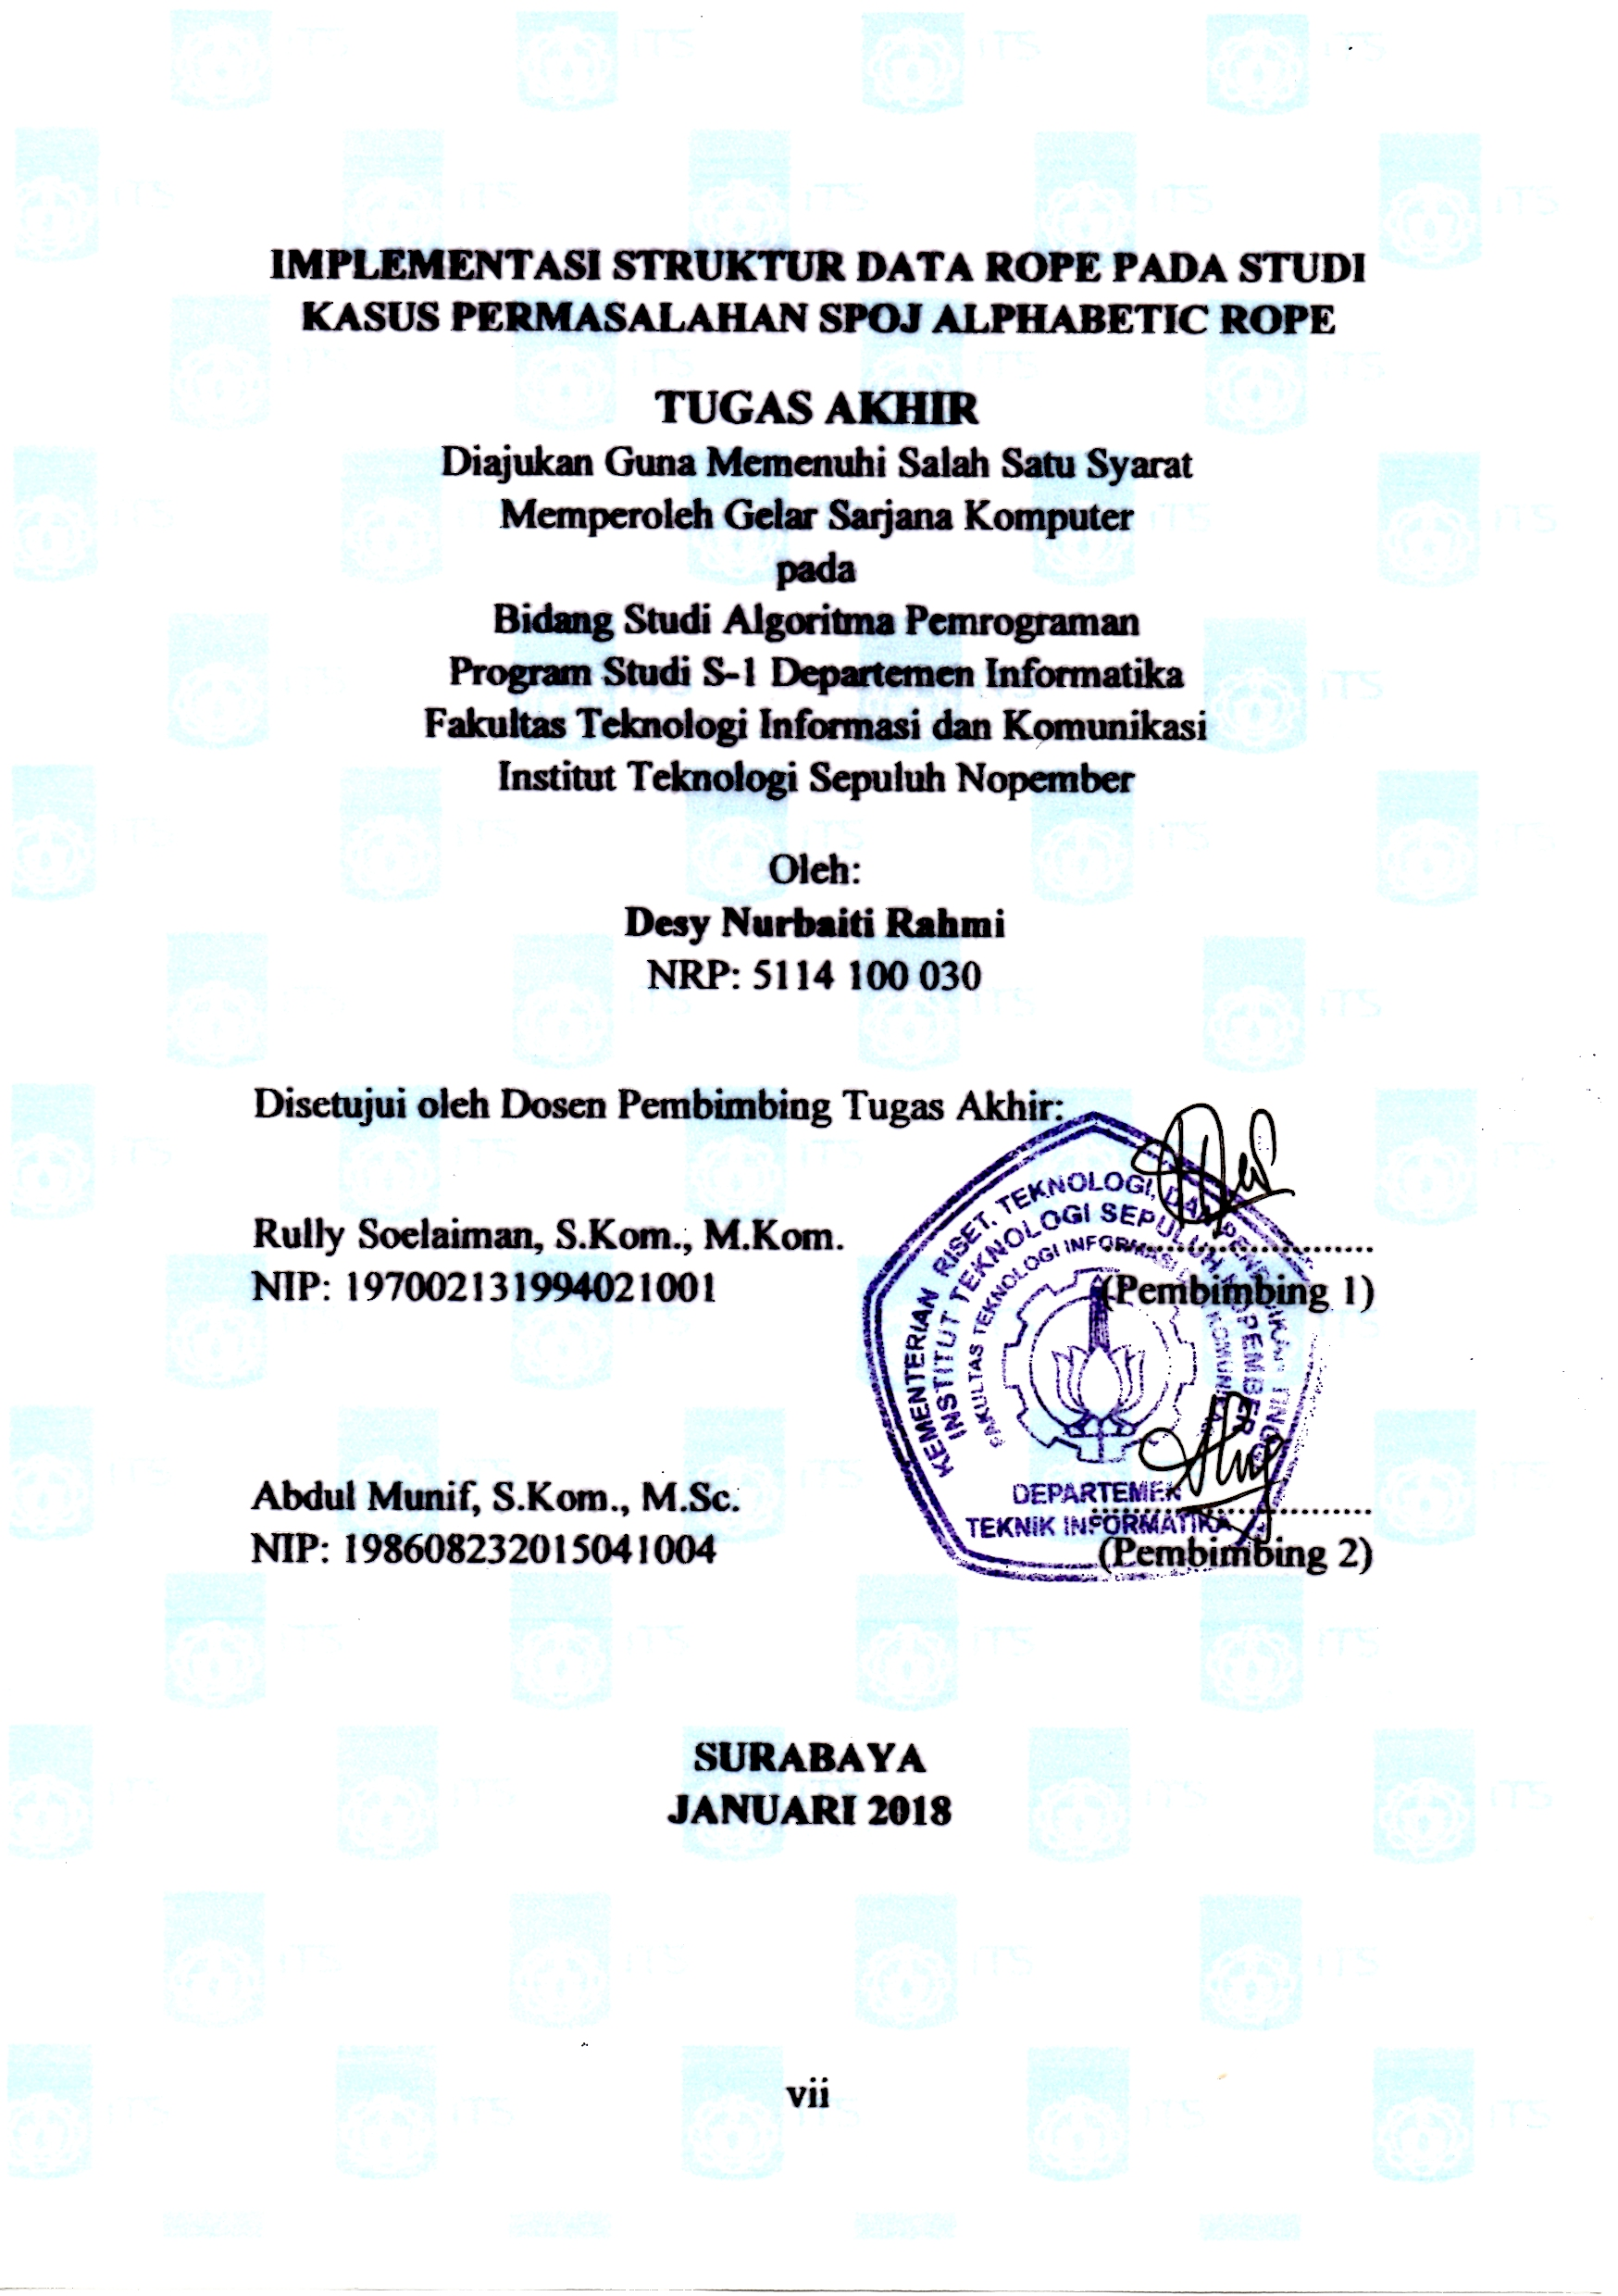
\includegraphics[scale=1]{pengesahan/pengesahan.png}}
		\label{figure:lpeng}
	\end{figure}
	
	\cleardoublepage
	% INDONESIAN ABSTRAK
\addcontentsline{toc}{chapter}{ABSTRAK}
\thispagestyle{plain}
\begin{centering}
\textbf{\MakeUppercase{\judul}}
\end{centering}

\begin{tabular}{ll}
Nama  & : \MakeUppercase{\penulis} \\
NRP & : \nrp \\
Departemen  & : \jurusan FTIF-ITS \\
Pembimbing I  & : \pembimbingSatu \\
Pembimbing II  & : \pembimbingDua
\end{tabular}
\\*[20pt]
\begin{centering}
\textbf{Abstrak}
\end{centering}
\itshape
% BEGIN
\\
\indent 
Permasalahan LIS and TREE merupakan sebuah permasalahan yang melibatkan sebuah struktur data tree. Dimana pada tree tersebut akan dicari LIS terpanjang dari seluruh simple path yang ada. Untuk menangani berbagai permasalahan pada permasalahan tersebut dibutuhkan struktur data yang mampu mendukung operasi-operasi tersebut dengan efisien.\\
Pada Tugas Akhir ini akan dirancang penyelesaian permasalahan LIS and TREE antara lain operasi pencarian nilai LIS pada node dan subtree saat ini, operasi update nilai LIS pada node dan subtree saat ini dan menggabungkan serta memindahkan nilai pada dua subtree yang berbeda. Struktur data klasik yang biasa digunakan dalam penyelesaian permasalahan ini merupakan salah satu jenis stuktur data Tree yaitu Segment Tree dengan menggabungkan konsep Disjoint Set Union.\\
Pada Tugas Akhir ini digunakan struktur data Segment Tree dan konsep Disjoint Set Union untuk menyelesaikan operasi-operasi tersebut.
% END
\rm \\
\textbf{Kata Kunci: Disjoint Set Union on Tree, Segment Tree, Longest Increasing Subsequence}


\cleardoublepage

% ENGLISH ABSTRACT
\addcontentsline{toc}{chapter}{ABSTRACT}
\thispagestyle{plain}
\begin{centering}
\textbf{\MakeUppercase{\judulEnglish}}
\end{centering}

\begin{tabular}{ll}
Name  & : \MakeUppercase{\penulis} \\
NRP & : \nrp \\
Major  & : \jurusanEnglish Faculty of IT-ITS \\
Supervisor I  & : \pembimbingSatu \\
Supervisor II  & : \pembimbingDua
\end{tabular}
\\*[20pt]
\begin{centering}
\textbf{Abstract}
\end{centering}
\itshape
% BEGIN
\\
\indent 
LIS and TREE is a problem which involves tree data structure. From that tree a LIS should be found from every simple path that exist. To handle various problem, an efficient data structure is needed to support the operations.\\
This undergraduate thesis will be designed problem solving for LIS and TREE such as operation to find LIS value in a subtree and node, operation to update value of LIS in a subtree and node, and also combine and transfer value of LIS between different subtree and node. Well known data structures, e.g tree specifically segment tree with combination of Disjoint Set Union concept is able to answer the problem efficiently.\\
In this undergraduate thesis Segment Tree data structure and Disjoint Set Union concept will be used to solve those operations.
\\
% END
\rm \\
\textbf{Keywords: Disjoint Set Union on Tree, Segment Tree, Longest Increasing Subsequence}

\cleardoublepage

	%\include{istilah/istilah}
	\chapter{KATA PENGANTAR}

\indent\indent Puji syukur Penulis panjatkan kepada Allah SWT. atas pimpinan, penyertaan, dan karunia-Nya sehingga Penulis dapat menyelesaikan Tugas Akhir yang berjudul :
\begin{center}
	\textbf{\MakeUppercase{\judul}}.
\end{center}

Penelitian Tugas Akhir ini dilakukan untuk memenuhi salah satu syarat meraih gelar Sarjana di Jurusan Teknik Informatika Fakultas Teknologi Informasi Institut Teknologi Sepuluh Nopember.

Dengan selesainya Tugas Akhir ini diharapkan apa yang telah dikerjakan Penulis dapat memberikan manfaat bagi perkembangan ilmu pengetahuan terutama di bidang teknologi informasi serta bagi diri Penulis sendiri selaku peneliti.

Penulis mengucapkan terima kasih kepada semua pihak yang telah memberikan dukungan baik secara langsung maupun tidak langsung selama Penulis mengerjakan Tugas Akhir maupun selama menempuh masa studi antara lain:

\begin{itemize}
	\item Papa, Mama dan keluarga Penulis yang selalu memberikan perhatian, dorongan dan kasih sayang yang menjadi semangat utama bagi diri Penulis sendiri baik selama penulis menempuh masa perkuliahan maupun pengerjaan Tugas Akhir ini.
	\item Bapak Rully Soelaiman, S.Kom., M.Kom. selaku Dosen Pembimbing yang telah banyak meluangkan waktu untuk memberikan ilmu, nasihat, motivasi, pandangan dan bimbingan kepada Penulis baik selama Penulis menempuh masa kuliah maupun selama pengerjaan Tugas Akhir ini.
	\item Bapak Abdul Munif, S.Kom., M.Sc. selaku dosen pembimbing yang telah memberikan ilmu, dan masukan kepada Penulis.
	\item Seluruh tenaga pengajar dan karyawan Jurusan Teknik Informatika ITS yang telah memberikan ilmu dan waktunya demi berlangsungnya kegiatan belajar mengajar di Jurusan Teknik Informatika ITS.
	\item Seluruh teman Penulis di Jurusan Teknik Informatika ITS yang telah memberikan dukungan dan semangat kepada Penulis selama Penulis menyelesaikan Tugas Akhir ini.
	\item Teman-teman, Kakak-kakak dan Adik-adik \textit{administrator} Laboratorium Algoritma dan Pemrograman yang selalu menjadi teman untuk berbagi ilmu.
\end{itemize}

Penulis mohon maaf apabila masih ada kekurangan pada Tugas Akhir ini. Penulis juga mengharapkan kritik dan saran yang membangun untuk pembelajaran dan perbaikan di kemudian hari. Semoga melalui Tugas Akhir ini Penulis dapat memberikan kontribusi dan manfaat yang sebaik-baiknya. \\ \\ \\

\hfill Surabaya, Juni \tahun \\ \\ \\

\hfill \penulis \\
\cleardoublepage

	\tableofcontents
	\cleardoublepage
	\listoftables
	\cleardoublepage
	\listoffigures
	\cleardoublepage
	\lstlistoflistings
	\cleardoublepage
	
	\mainmatter
	\chapter{PENDAHULUAN}
Pada bab ini akan dijelaskan latar belakang, rumusan masalah, batasan masalah, tujuan, manfaat, metodologi dan sistematika penulisan Tugas Akhir.

\section{\quad Latar Belakang}
\quad Di dalam ilmu komputer, terdapat permasalahan pengaplikasian struktur data yang tepat, guna memecahkan permasalahan yang ada. Hal ini dikarenakan banyaknya jenis struktur data dan kegunaannya yang beragam. Peneliti mencoba mencari beberapa permasalahan yang berkaitan dengan pengaplikasian struktur data dalam dunia pemrograman dan menemukan permasalahan di situs \textit{online} SPOJ. Di dalam situs tersebut terdapat sebuah permasalahan dengan nama \problem\cite{listree}.

\quad Pada permasalahan ini diberikan masukan berupa bilangan bulat yang disimbolkan N, yang merepresentasikan jumlah \textit{node} di sebuah \textit{tree}. Dari \textit{tree} tersebut diminta untuk mencari \textit{Longest Increasing Subsequence} (LIS).\\
Hasil Tugas Akhir ini diharapkan dapat memberi gambaran mengenai penerapan \textit{disjoint set union} pada struktur data \textit{tree}.

\section{\quad Rumusan Masalah}
\quad Rumusan masalah yang diangkat dalam Tugas Akhir ini adalah sebagai berikut:
\begin{enumerate}
	\item Bagaimana menyelesaikan \problem\cite{listree} pada situs penilaian SPOJ?
	\item Bagaimana menerapkan konsep \textit{disjoint set union} pada struktur data \textit{segment tree}?
	\item Bagaimana kinerja algoritma \textit{disjoint set union} pada struktur data \textit{segment tree} dalam menyelesaikan \problem\cite{listree}?
\end{enumerate}

\section{\quad Batasan Masalah}
\quad Permasalahan yang dibahas pada Tugas Akhir ini memiliki beberapa batasan, yaitu sebagai berikut:

\begin{enumerate}
	\item Implementasi algoritma menggunakan bahasa pemrograman C++.
	\item Besar ukuran berkas masukkan dalam sekali uji maksimal 2 MB.
	\item Banyak kasus uji disimbolkan T, dengan rentang $ 1 $ - $ 1000 $.
	\item Jumlah \textit{node} yang disimbolkan N berkisar antara $ 1 $ - $ 100.000 $.
	\item Berikutnya sebanyak N-1 baris diinputkan 2 angka disimbolkan a dan b dengan syarat a ≥ 1 dan b ≤ N, yang merepresentasikan bahwa vertex a terhubung dengan vertex b.
	\item Kombinasi dari vertex a dan b haruslah unik.
	\item Penyimpanan yang dibutuhkan dalam 1 kali percobaan kurang dari 1536 MB.
	\item Batas waktu pada program untuk setiap percobaan kurang dari $ 1 $ detik.

\end{enumerate}

\section{\quad Tujuan}
\quad Tujuan dari Tugas Akhir ini adalah sebagai berikut:
\begin{enumerate}
	\item Melakukan desain dan implementasi penyelesaian \problem\cite{listree} pada situs penilaian SPOJ.
	\item Menganalisis hasil kinerja penyelesaian \problem\cite{listree}.
\end{enumerate}

\section{\quad Metodologi}
\quad Ada beberapa tahap dalam proses pengerjaan tugas akhir ini, yaitu sebagai berikut:
\begin{enumerate}
	\item Studi Literatur\\
	Pada tahap ini, dilakukan studi mengenai pengimplementasian \textit{disjoint set union} pada struktur data \textit{segment tree} serta algoritman penyelesaian \textit{Longest Increasing Subsequence}. Sumber studi antara lain dari buku-buku literatur, situs-situs pembelajaran \textit{online}, dan materi kuliah yang bersangkutan.
	\item Implementasi\\
	Pada Tahap ini, akan dilakukan pembangunan dari algoritma yang telah dipelajari menjadi sebuah sistem yang dapat digunakan. Bahasa pemrograman yang digunakan adalah C++ dengan menggunakan IDE(\textit{Integrated Development System}) Dev-C++.
	\item Uji Coba\\
	Tahap ini merupakan tahap pengujian aplikasi dengan data masukan yang telah ditentukan untuk menguji kebenaran hasil implementasi algoritma serta menguji waktu eksekusi aplikasi untuk data masukan yang telah ditentukan. Pada tahap ini juga dilakukan optimasi dari hasil implementasi apabila aplikasi masih kurang efisien.
	\item Penyusunan buku tugas akhir\\
	Tahap ini merupakan tahap penyusunan laporan berupa buku tugas akhir sebagai dokumentasi pelaksanaan tugas akhir yang mencakup seluruh teori, implementasi serta hasil pengujian yang telah dikerjakan.\\\\
\end{enumerate}

	\section{\quad Sistematika Penulisan Laporan}
	\quad Berikut adalah sistematika penulisan buku Tugas Akhir ini:
	\begin{enumerate}
		\item BABI: PENDAHULUAN
		
		Bab ini berisi latar belakang, rumusan masalah, batasan masalah, tujuan, manfaat, metodologi dan sistematika penulisan Tugas Akhir.
		
		\item BAB II: DASAR TEORI
		
		Bab ini berisi dasar teori mengenai permasalahan dan algoritma penyelesaian yang digunakan dalam Tugas Akhir
		
		\item BAB III: DESAIN
		
		Bab ini berisi desain algoritma dan struktur data yang digunakan dalam penyelesaian permasalahan.
		
		\item BAB IV: IMPLEMENTASI
		
		Bab ini berisi implementasi berdasarkan desain algortima yang telah dilakukan pada tahap desain.
		
		\item BAB V: UJI COBA
		
		Bab ini berisi uji coba dan evaluasi dari hasil implementasi yang telah dilakukan pada tahap implementasi.
		
		\item BAB VI: PENUTUP
		
		Bab ini berisi kesimpulan dan saran yang didapat dari hasil uji coba yang telah dilakukan.
	\end{enumerate}

\cleardoublepage

	\chapter{DASAR TEORI}
Pada bab ini akan dijelaskan mengenai dasar teori yang menjadi dasar pengerjaan Tugas Akhir ini.

\section{\quad Deskripsi Umum Permasalahan}
\quad Permasalahan yang diangkat pada Tugas Akhir ini adalah mencari \textit{Longest Increasing Subsequence} (LIS) dari sebuah \textit{tree}, dimana \textit{node} dalam \textit{tree} tersebut sesuai dengan masukan yang diberikan, dan terdapat \textit{edge} yang saling menghubungkannya. Contoh masukan yang diberikan pada daring terlihat pada Tabel \ref{tabel:cont1}.

\begin{table}[H]
\centering
	\begin{tabular}{|p{2cm}|p{2cm}|}
		\hline
		2\\
		\hline
		12\\
		\hline
		1 8\\
		\hline
		8 6\\
		\hline
		8 3\\
		\hline
		3 12\\
		\hline
		3 10\\
		\hline
		3 5\\
		\hline
		5 4\\
		\hline
		5 2\\
		\hline
		1 9\\
		\hline
		9 11\\
		\hline
		9 7\\
		\hline
	\end{tabular}
	\caption{Contoh masukan dari daring \label{tabel:cont1}}
\end{table}
\quad Dari masukan tadi akan terbentuk sebuah \textit{tree} sesuai seperti angka yang telah dimasukan, visualisasi dari \textit{tree} dapat dilihat di Gambar \ref{fig:treedes}.

\begin{figure}[H]
	\centering
	\begin{tikzpicture}[level/.style={sibling distance = 5cm/#1, level distance = 1.5cm}, scale=0.68,transform shape]
	\node[treenode]{1}
	child{
		node[treenode]{8}
		child{
			node[treenode]{6}
		}
		child{
			node[treenode]{3}
			child{
				node[treenode]{12}
			}
			child{
				node[treenode]{10}
			}
			child{
				node[treenode]{5}
				child{
					node[treenode]{4}
				}
				child{
					node[treenode]{2}
				}
			}	
		}
	}
	child{
		node[treenode]{9}
		child{
			node[treenode]{11}
		}
		child{
			node[treenode]{7}
		}	
	};
	\end{tikzpicture}
	\caption{Bentuk akhir tree sesuai masukan dari daring\label{fig:treedes}}
\end{figure}
\quad Dari \textit{tree} tersebut akan dicari LIS sesuai dengan permasalahan soal, untuk contoh masukan tersebut keluaran LIS adalah $4$. Visualisasi jawaban terlihat pada Gambar \ref{fig:ansex}.

\begin{figure}[H]
	\centering
	\begin{tikzpicture}[level/.style={sibling distance = 5cm/#1, level distance = 1.5cm}, scale=0.68,transform shape]
	\node[treenode]{1}
	child{
		node[treenode,fill=green]{8}
		child{
			node[treenode]{6}
		}
		child{
			node[treenode,fill=green]{3}
			child{
				node[treenode]{12}
			}
			child{
				node[treenode]{10}
			}
			child{
				node[treenode]{5}
				child{
					node[treenode]{4}
				}
				child{
					node[treenode,fill=green]{2}
				}
			}	
		}
	}
	child{
		node[treenode,fill=green]{9}
		child{
			node[treenode,fill=green]{11}
		}
		child{
			node[treenode]{7}
		}	
	};
	\end{tikzpicture}
	\caption{\textit{Vertex} dengan warna hijau menunjukkan \textit{node} yang menjadi anggota LIS.\label{fig:ansex}}
\end{figure}


\section{\quad \textit{Longest Increasing Subsequence}}
\quad Dalam ilmu komputer, permasalahan \textit{Longest Increasing Subsequence} atau yang biasa disingkat menjadi LIS, merupakan permasalahan yang bertujuan untuk menemukan \textit{subsequence} terpanjang dari sebuah \textit{sequence} dimana \textit{subsequence} tersebut memiliki elemen yang sudah disortir dari nilai terkecil ke terbesar.\\
Untuk dapat menyelesaikannya algoritma yang dibutuhkan adalah sebagai berikut:

\quad Dimisalkan terdapat sebuah \textit{array} bernama $A[]$ yang memiliki panjang tertentu, dan penulis juga memiliki LIS terpanjang sementara atau disebut \textit{active list} dengan panjang tertentu. Kemudian penulis ingin menambahkan elemen ke-\textit{i} atau $A[\textit{i}]$ maka harus memperhatikan beberapa hal sebagai berikut\cite{LIS}:
\begin{enumerate}
	\item jika $A[\textit{i}]$ adalah elemen terkecil dari \textit{active list} maka buat \textit{active list} baru dengan panjang $1$.
	\item Jika $A[\textit{i}]$ adalah elemen terbesar dari \textit{active list} maka lakukan duplikasi terhadap \textit{active list} terpanjang dan tambahkan elemen tersebut di akhir.
	\item Jika $A[\textit{i}]$ bukan elemen terbesar ataupun terkecil maka cari \textit{active list} dengan elemen terakhir yang terbesar dan lebih kecil dari $A[\textit{i}]$, lakukan duplikasi dan tambahkan elemen tersebut, dan hapus \textit{list} lain dengan panjang yang sama.
\end{enumerate}
\textbf{Contoh}\\
Untuk menemukan LIS dari array $A[0,8,4,12,2,10,14]$
\begin{enumerate}
	\item $A[0]$ = $1$, karena merupakan elemen pertama dan belum ada \textit{active list} maka masuk ke \textit{case} 1.\\\\
	$[0]$\\
	\item $A[1]$ = $8$, karena angka $8$ lebih besar daripada $0$, maka masuk ke \textit{case} 2.\\\\
	$[0]$\\
	$[0,8]$\\
	\item $A[2]$ = $4$, karena angka $4$ berada di antara $0$ dan $8$, maka akan masuk ke \textit{case} 3.\\\\
	$[0]$\\
	$[0,4]$\\
	\sout{$[0,8]$} (dihilangkan)\\
	\item $A[3]$ = $12$, karena angka $12$ lebih besar daripada $4$, maka masuk ke \textit{case} 1.\\\\
	$[0]$\\
	$[0,4]$\\
	$[0,4,12]$\\\\
	\item $A[4]$ = $2$, karena angka $2$ berada di antara $0$ dan $12$ maka akan masuk ke \textit{case} 3.\\\\
	$[0]$\\
	$[0,2]$\\
	\sout{$[0,4]$} (dihilangkan)\\
	$[0,4,12]$\\
	\item $A[5]$ = $10$, karena angka $10$ berada di antara $0$ dan $12$ maka akan masuk ke \textit{case} 3.\\\\
	$[0]$\\
	$[0,2]$\\
	$[0,2,10]$\\
	\sout{$[0,4,12]$} (dihilangkan)\\
	\item $A[6]$ = $14$, karena angka $14$ lebih besar daripada $10$ maka akan masuk ke \textit{case} 1.\\\\
	$[0]$\\
	$[0,2]$\\
	$[0,2,10]$\\
	$[0,2,10,14]$\\ merupakan LIS dari array tersebut.
\end{enumerate}

\section{\quad \textit{Binary Tree}}
\quad \textit{Binary Tree} merupakan salah satu jenis struktur data \textit{Tree}, yang memiliki maksimal hanya dua \textit{child} untuk setiap \textit{node} yang ada, kedua \textit{child} tersebut biasa disebut dengan istilah \textit{left child} dan \textit{right child}. Gambar \ref{fig:bt} menunjukkan contoh dari \textit{binary tree}.
\begin{figure}[H]
	\centering
	\begin{tikzpicture}[level/.style={sibling distance = 5cm/#1, level distance = 1.5cm}, scale=0.68,transform shape]
	\node[treenode]{}
	child{
		node[treenode]{}
		child{
			node[treenode]{}
		}
		child{
			node[treenode]{}
		}
	}
	child{
		node[treenode]{}
		child{
			node[treenode]{}
		}
		child{
			node[treenode]{}
		}
	};
	\end{tikzpicture}
	\caption{Visualisasi dari bentuk struktur data \textit{Binary Tree}.}\label{fig:bt}
\end{figure}

\section{\quad \textit{Segment Tree}}
\quad\textit{Segment Tree} merupakan salah satu jenis struktur data yang merepresentasikan suatu nilai yang terhubung dengan suatu jeda atau interval tertentu di dalam \textit{array}\cite{ST}.

\quad Dimisalkan terdapat sebuah struktur data \textit{segment tree} yang menyimpan interval untuk suatu \textit{array} $A[]$ dengan panjang $n$.Maka rumusan algoritma yang dapat digunakan untuk konstruksi \textit{segment tree} sebagai berikut\cite{ST2}:
\begin{enumerate}
	\item Buat node yang berisikan seluruh elemen \textit{array} $A[]$.
	\item Jika elemen di dalam node beranggotakan lebih dari satu, maka buat $2$ \textit{child node} baru yang beranggotakan elemen $A[0,... .,n/2]$ dan $A[(n/2)+1,... .,n]$.
	\item Jika elemen di dalam node hanya beranggotakan 1 elemen maka proses dihentikan.
\end{enumerate}
\quad Pada Gambar \ref{fig:subbentukST1} menunjukkan  \textit{node} yang menyimpan nilai dari seluruh rentang yang ada menjadi \textit{root} dari \textit{segment tree}.
\begin{figure}[H]
	\begin{subfigure}{.5\textwidth}
		\centering
		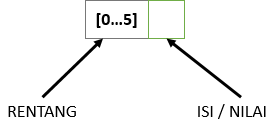
\includegraphics[scale=0.45]{assets/images/pembentukan_ST_1.PNG}
		\caption{}
		\label{fig:subbentukST1}
	\end{subfigure}
	\begin{subfigure}{.5\textwidth}
		\centering
		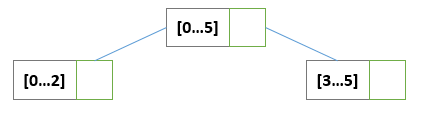
\includegraphics[scale=0.45]{assets/images/pembentukan_ST_2.PNG}
		\caption{}
		\label{fig:subbentukST2}
	\end{subfigure}
	\begin{subfigure}{.5\textwidth}
		\centering 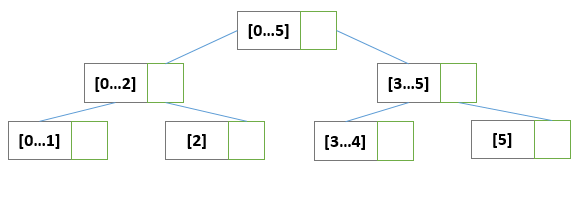
\includegraphics[scale=0.3]{assets/images/pembentukan_ST_3.PNG}
		\caption{}
		\label{fig:subbentukST3}
	\end{subfigure}
		\begin{subfigure}{.5\textwidth}
			\centering
			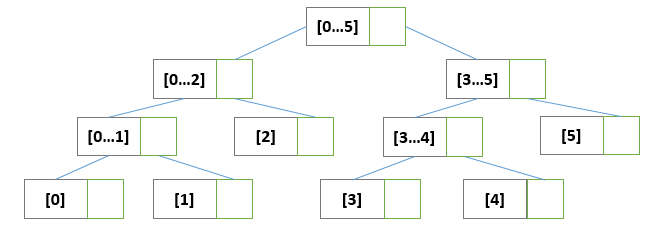
\includegraphics[scale=0.3]{assets/images/pembentukan_ST_4.PNG}
			\caption{}
			\label{fig:subbentukST4}
		\end{subfigure}	
	\caption{Proses pembentukan \textit{Segment Tree}}
	\label{fig:bentukST1}
\end{figure}
\quad Pada Gambar \ref{fig:subbentukST2} menunjukkan proses rekursi untuk membuat dua \textit{child} baru, \textit{child} kiri menyimpan nilai dari rentang 0 hingga 2, \textit{child} kanan menyimpan nilai dari rentang 3 hingga 5.

\quad Pada Gambar \ref{fig:subbentukST3} menunjukkan lanjutan proses rekursi lagi, namun untuk \textit{node} yang menyimpan hanya satu rentang saja, yaitu \textit{node} yang menyimpan rentang 2 dan 5 proses dihentikan, bentuk akhir dari \textit{segment tree} terlihat pada Gambar \ref{fig:subbentukST4}

\quad Selain itu pada umumnya struktur data \textit{segment tree} juga memiliki fungsi \textit{$query()$} untuk mengambil nilai dari suatu rentang dan juga \textit{$update()$} untuk merubah nilai pada suatu rentang.
\quad Algoritma untuk melakukan fungsi \textit{$query()$} sebagai berikut:
\begin{enumerate}
	\item Cek apakah nilai dari rentang yang diinginkan berada dalam rentang saat ini.
	\item Jika iya ambil nilai yang berada di rentang tersebut.
	\item Jika tidak lakukan rekursi ke \textit{left child} dan \textit{right child}.
\end{enumerate}
\quad Untuk visualisasi proses \textit{$query()$} akan diambil nilai pada rentang $1$ sampai $4$. Pada Gambar \ref{fig:subqueryST1} proses dimulai dengan melakukan cek pada \textit{root} apakah rentang yang diinginkan masih termasuk atau tidak, \textit{root} menyimpan nilai dari rentang $0$ hingga $5$, maka rentang yang diinginkan masih termasuk didalamnya, dilakukan proses rekursi ke \textit{child}.
\begin{figure}[H]
	\begin{subfigure}{.5\textwidth}
		\centering
		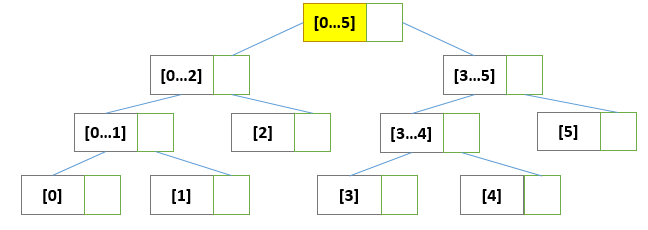
\includegraphics[scale=0.3]{assets/images/Query_ST_1.PNG}
		\caption{}
		\label{fig:subqueryST1}
	\end{subfigure}
	\begin{subfigure}{.5\textwidth}
		\centering
		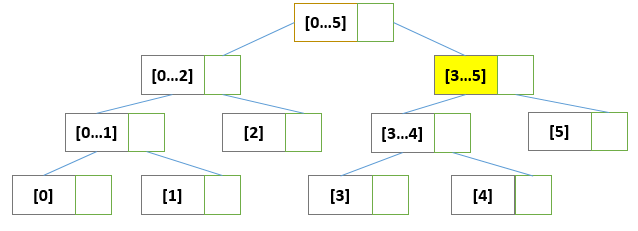
\includegraphics[scale=0.3]{assets/images/Query_ST_2.PNG}
		\caption{}
		\label{fig:subqueryST2}
	\end{subfigure}
	\begin{subfigure}{.5\textwidth}
		\centering 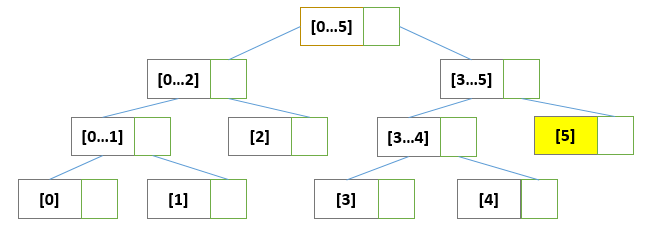
\includegraphics[scale=0.3]{assets/images/Query_ST_3.PNG}
		\caption{}
		\label{fig:subqueryST3}
	\end{subfigure}
	\begin{subfigure}{.5\textwidth}
		\centering
		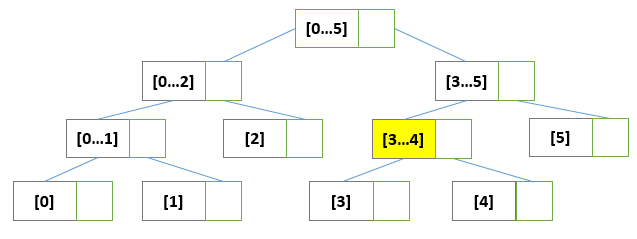
\includegraphics[scale=0.3]{assets/images/Query_ST_4.PNG}
		\caption{}
		\label{fig:subqueryST4}
	\end{subfigure}	
	\caption{Proses rekursi \textit{$query$} pada \textit{right child} dari \textit{Segment Tree} }
	\label{fig:queryST1}
\end{figure}
\quad Pada Gambar \ref{fig:subqueryST2} dilakukan pengecekan pada \textit{node} yang menyimpan rentang nilai $3$ hingga $5$, karena masih mencakup rentang yang dicari maka dilanjutkan proses rekursi pada \textit{child node} tersebut. 

\quad Pada Gambar \ref{fig:subqueryST3} proses dilakukan pada \textit{node} yang menyimpan rentang nilai $5$ saja, karena rentang tersebut tidak dicari, maka proses pada \textit{node} tersebut dihentikan. Pada Gambar \ref{fig:subqueryST4} dilakukan pengecekan pada \textit{node} yang menyimpan rentang nilai $3$ hingga $4$, dimana \textit{node} tersebut menyimpan nilai sesuai dengan rentang yang diinginkan, maka akan diambil nilainya dan dibandingkan dengan \textit{sibling} dari \textit{node} tersebut, untuk kemudian diambil nilai maksimum atau minimum sesuai kebutuhan.

\quad Rekursi dilanjutkan ke \textit{child} yang berada pada sisi kiri dari \textit{root}. Pada Gambar \ref{fig:subqueryST5} proses dilakukan pada \textit{node} yang menyimpan rentang nilai dari rentang $0$ hingga $2$, dikarenakan rentang tersebut mencakup rentang yang diinginkan didalamnya, maka dilakukan proses rekursi ke \textit{child node} tersebut.
\begin{figure}[H]
	\begin{subfigure}{.5\textwidth}
		\centering
		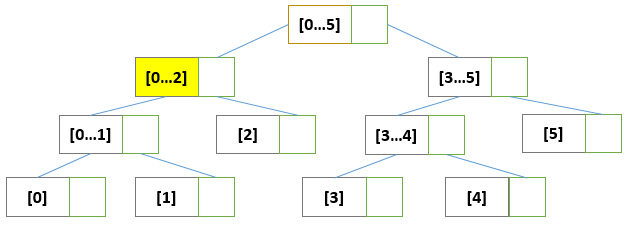
\includegraphics[scale=0.3]{assets/images/Query_ST_5.PNG}
		\caption{}
		\label{fig:subqueryST5}
	\end{subfigure}
	\begin{subfigure}{.5\textwidth}
		\centering
		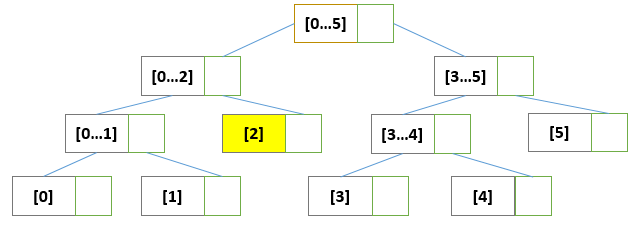
\includegraphics[scale=0.3]{assets/images/Query_ST_6.PNG}
		\caption{}
		\label{fig:subqueryST6}
	\end{subfigure}
	\begin{subfigure}{.5\textwidth}
		\centering 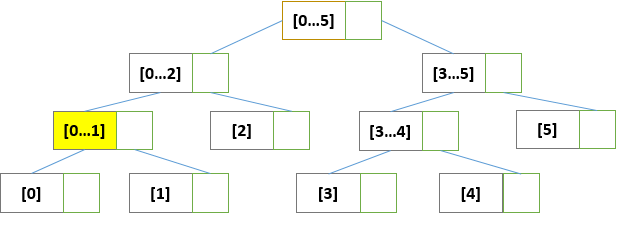
\includegraphics[scale=0.3]{assets/images/Query_ST_7.PNG}
		\caption{}
		\label{fig:subqueryST7}
	\end{subfigure}
	\begin{subfigure}{.5\textwidth}
		\centering
		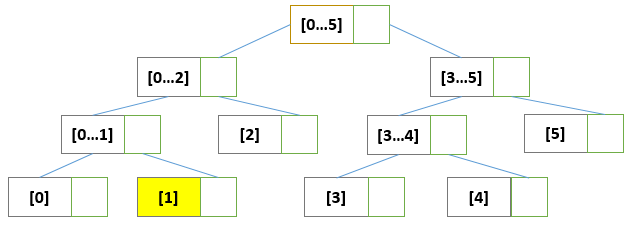
\includegraphics[scale=0.3]{assets/images/Query_ST_8.PNG}
		\caption{}
		\label{fig:subqueryST8}
	\end{subfigure}	
	\caption{Proses rekursi \textit{$query$} pada \textit{left child} dari \textit{Segment Tree}}
	\label{fig:queryST2}
\end{figure}
\quad Pada Gambar \ref{fig:subqueryST6}, karena \textit{node} tersebut termasuk pada rentang yang diinginkan maka nilai didalamnya akan diambil, untuk dibandingkan dengan \textit{sibling} dari \textit{node} tersebut nantinya. Proses dilanjutkan ke \textit{node} yang menyimpan rentang $0$ hingga $1$, seperti pada Gambar \ref{fig:subqueryST7}.

\quad Pada Gambar \ref{fig:subqueryST8} dilakukan pengecekan pada \textit{node} yang menyimpan rentang nilai $1$, dimana \textit{node} tersebut menyimpan nilai sesuai dengan rentang yang diinginkan. Sedangkan pada Gambar \ref{fig:subqueryST9}, nilai pada rentang $0$ tidak termasuk nilai yang diinginkan. 
\begin{figure}[H]
	\begin{subfigure}{.5\textwidth}
		\centering
		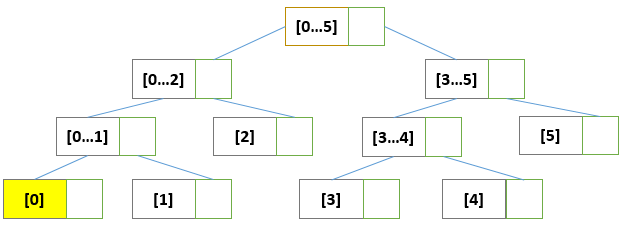
\includegraphics[scale=0.3]{assets/images/Query_ST_9.PNG}
		\caption{}
		\label{fig:subqueryST9}
	\end{subfigure}
	\begin{subfigure}{.5\textwidth}
		\centering
		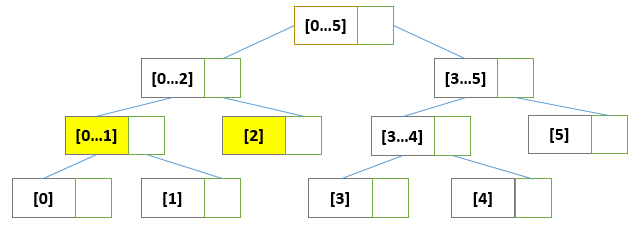
\includegraphics[scale=0.3]{assets/images/Query_ST_10.PNG}
		\caption{}
		\label{fig:subqueryST10}
	\end{subfigure}
	\begin{subfigure}{.5\textwidth}
		\centering 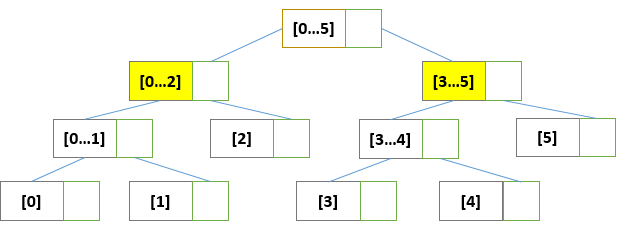
\includegraphics[scale=0.3]{assets/images/Query_ST_11.PNG}
		\caption{}
		\label{fig:subqueryST11}
	\end{subfigure}
	\begin{subfigure}{.5\textwidth}
		\centering
		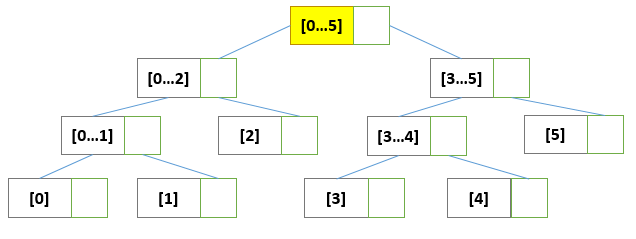
\includegraphics[scale=0.3]{assets/images/Query_ST_12.PNG}
		\caption{}
		\label{fig:subqueryST12}
	\end{subfigure}	
	\caption{Proses pengembalian nilai \textit{$query$} ke \textit{root} pada \textit{Segment Tree}}
	\label{fig:queryST3}
\end{figure}
\quad Sebelum mengembalikan nilai ke atas, akan dilakukan perbandingan nilai, dengan \textit{sibling node} tersebut, untuk mengambil nilai yang maksimum atau minimum sesuai dengan kebutuhan, proses ini terlihat pada Gambar \ref{fig:subqueryST10} dan \ref{fig:subqueryST10}. Pada akhirnya nilai yang dicari akan berada pada \textit{root}, terlihat pada Gambar \ref{fig:subqueryST12}, menandakan bahwa proses \textit{$query()$} telah selesai.
 
\quad Algoritma untuk melakukan fungsi \textit{$update()$} sebagai berikut:
\begin{enumerate}
	\item Cek apakah nilai dari rentang yang diinginkan berada dalam rentang saat ini.
	\item Jika iya ambil \textit{update} nilai yang berada di rentang tersebut.
	\item Jika tidak lakukan rekursi ke \textit{left child} dan \textit{right child}.
\end{enumerate} 
\quad Sebagai contoh akan dilakukan \textit{$update()$} pada \textit{node} yang menyimpan nilai rentang $4$. Awal proses dimulai dengan melakukan pengecekan pada \textit{root}, seperti yang terlihat pada Gambar \ref{fig:subupdateST1}. Karena di dalam \textit{root} mencakup rentang yang ingin diupdate, maka dilakukan rekursi ke \textit{child}.
\begin{figure}[H]
	\begin{subfigure}{.5\textwidth}
		\centering
		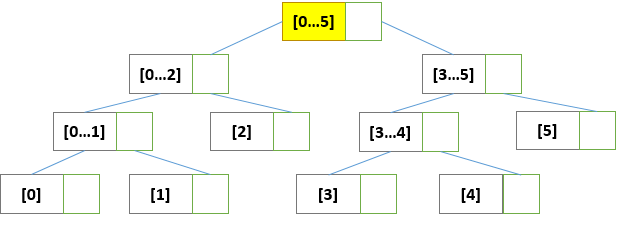
\includegraphics[scale=0.3]{assets/images/Update_ST_1.PNG}
		\caption{}
		\label{fig:subupdateST1}
	\end{subfigure}
	\begin{subfigure}{.5\textwidth}
		\centering
		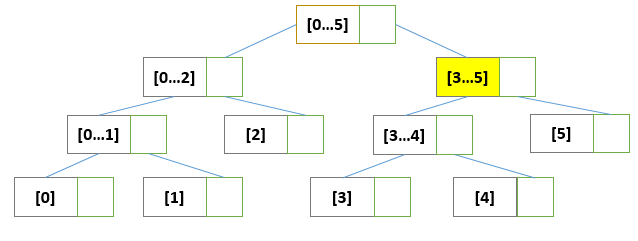
\includegraphics[scale=0.3]{assets/images/Update_ST_2.PNG}
		\caption{}
		\label{fig:subupdateST2}
	\end{subfigure}
	\begin{subfigure}{.5\textwidth}
		\centering
		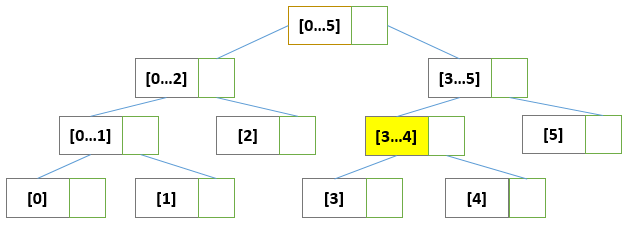
\includegraphics[scale=0.3]{assets/images/Update_ST_3.PNG}
		\caption{}
		\label{fig:subupdateST3}
	\end{subfigure}
	\begin{subfigure}{.5\textwidth}
		\centering
		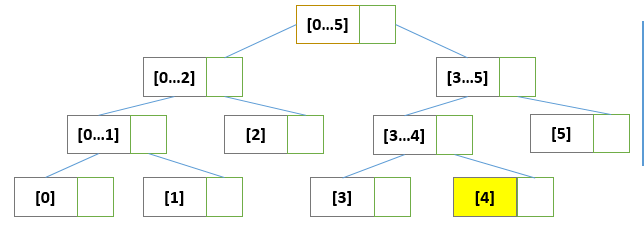
\includegraphics[scale=0.3]{assets/images/Update_ST_4.PNG}
		\caption{}
		\label{fig:subupdateST4}
	\end{subfigure}
	\caption{Proses pencarian \textit{node} untuk melakukan \textit{$update$} pada \textit{Segment Tree}}
	\label{fig:updateST1}
\end{figure}
\quad Karena \textit{left child} dari \textit{root} tidak menyimpan nilai dari rentang yang diinginkan maka proses pada \textit{left child} tidak dilanjutkan. Sedangkan di dalam \textit{right child} dari \textit{root} menyimpan rentang yang diinginkan, maka akan dilakukan rekursi pada \textit{right child}, seperti pada Gambar \ref{fig:subupdateST2}. Pada Gambar \ref{fig:subupdateST3} proses dilanjutkan, karena \textit{node} tersebut masih menyimpan rentang yang diinginkan, maka proses rekursi dilanjutkan ke \textit{child}nya. Pada Gambar \ref{fig:subupdateST4} proses telah mencapai \textit{node} dengan rentang diinginkan, maka akan dilakukan perubahan pada nilai yang disimpan didalamnya. \newpage
\quad Setelah nilai telah diubah, maka sebelum mengembalikan nilai ke \textit{parent}nya akan dilakukan perbandingan nilai dengan \textit{node} yang menjadi \textit{sibling}nya untuk mengambil nilai maksimum atau minimum sesuai dengan kebutuhan, proses ini terlihat pada Gambar \ref{fig:subupdateST5} dan \ref{fig:subupdateST6}, hingga akhirnya nilai kembali pada \textit{root} seperti pada Gambar \ref{fig:subupdateST7}.
\begin{figure}[H]
	\begin{subfigure}{.5\textwidth}
		\centering
		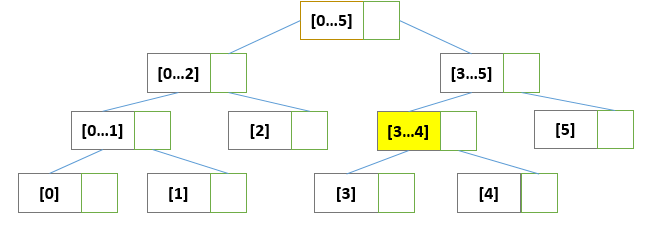
\includegraphics[scale=0.3]{assets/images/Update_ST_5.PNG}
		\caption{}
		\label{fig:subupdateST5}
	\end{subfigure}
	\begin{subfigure}{.5\textwidth}
		\centering
		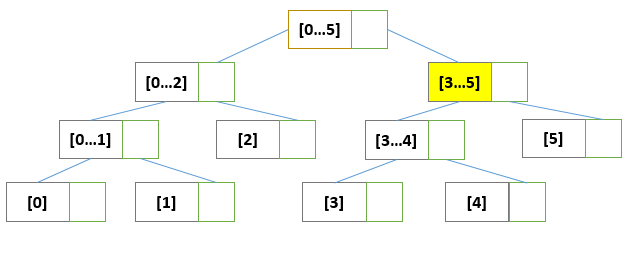
\includegraphics[scale=0.3]{assets/images/Update_ST_6.PNG}
		\caption{}
		\label{fig:subupdateST6}
	\end{subfigure}
	\begin{subfigure}{1.0\textwidth}
		\centering
		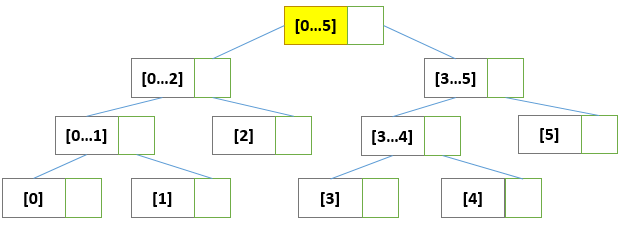
\includegraphics[scale=0.3]{assets/images/Update_ST_7.PNG}
		\caption{}
		\label{fig:subupdateST7}
	\end{subfigure}
	\caption{Proses pengembalian nilai hasil \textit{$update$} pada \textit{Segment Tree}}
	\label{fig:updateST2}
\end{figure}
\section{\quad \textit{Heavy-Light Decomposition}}
\quad\textit{Heavy-Light Decomposition} adalah teknik dekomposisi sebuah \textit{tree} menjadi sebuah \textit{disjoint chains} (tidak ada 2 \textit{chain} yang memiliki \textit{node} yang sama). Disebut \textit{Heavy-Light} karena dekomposisi dilakukan berdasarkan kriteria yang telah ditentukan untuk membedakan apakah \textit{chain} tersebut merupakan \textit{node heavy} atau \textit{light}.

\quad Penggunaan konsep \textit{Heavy-Light Decomposition}, yakni mengumpamakan sebuah \textit{node} mempunyai satu \textit{special child} yang merupakan sebuah \textit{subtree} dengan ukuran paling besar di antara \textit{child} lainnya. sehingga dapat diumpamakan \textit{tree} yang telah dibuat terdiri dari beberapa \textit{chain} dimana setiap \textit{chain} mempunyai \textit{head} yang bukan merupakan \textit{special child} dari \textit{parent child} tersebut.

\quad Setelah membentuk \textit{tree}, selanjutnya dicatat \textit{edge} mana yang merupakan \textit{heavy edge} dan \textit{light edge}. Dengan aturan berikut:
\begin{enumerate}
	\item \textit{Heavy edge} adalah \textit{edge} dengan jumlah \textit{child} lebih besar atau sama dengan setengah jumlah \textit{child} dari \textit{parent child} tersebut.
	\item \textit{Light edge} adalah \textit{edge} dengan jumlah \textit{child} kurang dari setengah jumlah \textit{child} dari \textit{parent child} tersebut.
\end{enumerate}
\quad Pada Gambar \ref{fig:ht} dapat dilihat terdapat banyak warna berbeda, setiap warna menggambarkan \textit{chain} yang berbeda, dan \textit{heavy chain} untuk \textit{tree} tersebut ditandai dengan warna hijau.
\begin{figure}[H]
\centering
\begin{tikzpicture}[level/.style={sibling distance = 5cm/#1, level distance = 1.5cm}, scale=0.68,transform shape]
	\node[treenode,fill=green]{1}
	child{
		node[treenode,fill=green]{2}
		child{
			node[treenode,fill=yellow]{5}
		}
		child{
			node[treenode,fill=green]{6}
			child{
				node[treenode,fill=green]{8}
				child{
					node[treenode,fill=green]{10}
					}
				child{
					node[treenode,fill=brown]{11}
					}
				}
		}
	}
	child{
		node[treenode,fill=cyan]{3}
		child{
			node[treenode,fill=cyan]{7}
			child{
				node[treenode,fill=cyan]{9}
			}
		}
	}
	child{
		node[treenode,fill=pink]{4}
		};
\end{tikzpicture}
\caption{Contoh penggambaran \textit{Heavy-Light Decomposition}\label{fig:ht}}
\end{figure}

\section{\quad \textit{Disjoint Set Union}}
\quad Struktur data \textit{disjoint set} adalah sebuah struktur data yang menyimpan sekumpulan himpunan atau \textit{set}. Dua himpunan bisa disebut \textit{disjoint} jika kedua himpunan tersebut tidak memiliki perpotongan, atau perpotongannya sama dengan $\textit{null}$. Sebagai contoh himpunan $\{1,2\}$ dan $\{3,4\}$ merupakan himpunan yang \textit{disjoint} karena tidak memiliki elemen yang sama diantara keduanya.

\quad \textit{Disjoint set union} sendiri merupakan suatu algoritma yang digunakan untuk menyatukan himpunan yang \textit{disjoint} dengan himpunan lainnya. Hal ini dapat dilakukan dengan melakukan operasi \textit{$merge(a,b)$}, dimana $a$ dan $b$ adalah dua himpunan yang saling \textit{disjoint}.

\textbf{Contoh}:\\
\quad Dimisalkan terdapat $5$ buah himpunan bagian yang memiliki anggota berjumlah $1$ yaitu: $\{1\}$, $\{2\}$, $\{3\}$, $\{4\}$, dan $\{5\}$. Kemudian dilakukan operasi seperti pada Tabel \ref{tabel:visdsu1} dan \ref{tabel:visdsu2}.
\begin{table}[H]
	\begin{tabular}{|p{0.25cm}|p{2.5cm}|p{3.5cm}|p{2.5cm}|}
		\hline
		No & Operasi & Visualisasi Himpunan & Keterangan\\
		\hline
		1 & Kondisi Awal & \centering
		\begin{tikzpicture}
		[level/.style={sibling distance = 1.5cm/#1, level distance = 1.5cm}, scale=0.6,transform shape]
		\node[treenode]{1};
		\addvmargin{10mm}
		\end{tikzpicture}
		\begin{tikzpicture}
		[level/.style={sibling distance = 1.5cm/#1, level distance = 1.5cm}, scale=0.6,transform shape]
		\node[treenode]{2};
		\addvmargin{10mm}
		\end{tikzpicture}
		\begin{tikzpicture}
		[level/.style={sibling distance = 1.5cm/#1, level distance = 1.5cm}, scale=0.6,transform shape]
		\node[treenode]{3};
		\addvmargin{10mm}
		\end{tikzpicture}
		\begin{tikzpicture}
		[level/.style={sibling distance = 1.5cm/#1, level distance = 1.5cm}, scale=0.6,transform shape]
		\node[treenode]{4};
		\addvmargin{10mm}
		\end{tikzpicture}
		\begin{tikzpicture}
		[level/.style={sibling distance = 1.5cm/#1, level distance = 1.5cm}, scale=0.6,transform shape]
		\node[treenode]{5};
		\addvmargin{10mm}
		\end{tikzpicture} & Kondisi awal himpunan.
		\\ \hline
		2 & $merge(2,1)$ & \centering
		\begin{tikzpicture}
		[level/.style={sibling distance = 1.5cm/#1, level distance = 1.5cm}, scale=0.6,transform shape]
		\node[treenode]{1}
		child{
			node[treenode]{2}
		};
		\addvmargin{10mm}
		\end{tikzpicture}
		\begin{tikzpicture}
		[level/.style={sibling distance = 1.5cm/#1, level distance = 1.5cm}, scale=0.6,transform shape]
		\node[treenode]{3};
		\addvmargin{10mm}
		\end{tikzpicture}
		\begin{tikzpicture}
		[level/.style={sibling distance = 1.5cm/#1, level distance = 1.5cm}, scale=0.6,transform shape]
		\node[treenode]{4};
		\addvmargin{10mm}
		\end{tikzpicture}
		\begin{tikzpicture}
		[level/.style={sibling distance = 1.5cm/#1, level distance = 1.5cm}, scale=0.6,transform shape]
		\node[treenode]{5};
		\addvmargin{10mm}
		\end{tikzpicture} & Kondisi setelah $merge(2,1)$.
		\\ \hline
	\end{tabular}\caption{Visualisasi Himpunan bagian dan proses \textit{$merge()$} bagian 1. \label{tabel:visdsu1}}
\end{table}
\hspace{-2cm}
\begin{table}[H]
	\begin{tabular}{|p{0.25cm}|p{2.5cm}|p{3.5cm}|p{2.5cm}|}
		\hline
		3 & $merge(4,3)$ & \centering
		\begin{tikzpicture}
		[level/.style={sibling distance = 1.5cm/#1, level distance = 1.5cm}, scale=0.6,transform shape]
		\node[treenode]{1}
		child{
			node[treenode]{2}
		};
		\addvmargin{10mm}
		\end{tikzpicture}
		\begin{tikzpicture}
		[level/.style={sibling distance = 1.5cm/#1, level distance = 1.5cm}, scale=0.6,transform shape]
		\node[treenode]{3}
		child{
			node[treenode]{4}
		};
		\addvmargin{10mm}
		\end{tikzpicture}
		\begin{tikzpicture}
		[level/.style={sibling distance = 1.5cm/#1, level distance = 1.5cm}, scale=0.6,transform shape]
		\node[treenode]{5};
		\addvmargin{10mm}
		\end{tikzpicture} & Kondisi setelah $merge(4,3)$
		\\ \hline
		4 & $merge(3,1)$ & \centering
		\begin{tikzpicture}
		[level/.style={sibling distance = 1.5cm/#1, level distance = 1.5cm}, scale=0.6,transform shape]
		\node[treenode]{1}
		child{
			node[treenode]{2}
		}
		child{
			node[treenode]{3}
			child{
				node[treenode]{4}
			}
		};
		\addvmargin{10mm}
		\end{tikzpicture}
		\begin{tikzpicture}
		[level/.style={sibling distance = 1.5cm/#1, level distance = 1.5cm}, scale=0.6,transform shape]
		\node[treenode]{5};
		\addvmargin{10mm}
		\end{tikzpicture} & Kondisi setelah $merge(3,1)$
		\\ \hline
		5 & $merge(5,2)$ & \centering
		\begin{tikzpicture}
		[level/.style={sibling distance = 1.5cm/#1, level distance = 1.5cm}, scale=0.6,transform shape]
		\node[treenode]{1}
		child{
			node[treenode]{2}
			child{
				node[treenode]{5}
			}
		}
		child{
			node[treenode]{3}
			child{
				node[treenode]{4}
			}
		};
		\addvmargin{10mm}
		\end{tikzpicture} & Kondisi setelah $merge(5,2)$
		\\ \hline
	\end{tabular}
	\caption{Visualisasi Himpunan bagian dan proses \textit{$merge()$} bagian 2. \label{tabel:visdsu2}}
\end{table}
\section{\quad \textit{Preorder Numbering}}
\quad \textit{Preorder} merupakan salah satu metode \textit{traversing} sebuah \textit{tree}, yang juga merupakan bagian dari algoritma \textit{Depth-First Search} (DFS), yaitu sebuah algoritma yang mencari \textit{depth} atau kedalaman sedalam mungkin pada setiap \textit{child} sebelum melanjutkan ke \textit{sibling} selanjutnya.

\quad Algoritma dari \textit{preorder} adalah sebagai berikut:
\begin{enumerate}
	\item Cek apakah \textit{node} saat ini kosong
	\item Tampilkan nilai/data dari \textit{node} saat ini.
	\item Lakukan \textit{traverse} ke \textit{child} sebelah kiri secara rekursif.
	\item Lakukan \textit{traverse} ke \textit{child} sebelah kanan secara rekursif.
\end{enumerate}
\quad Visualisasi dari \textit{preorder} dapat dilihat pada Gambar \ref{fig:preorder}.
\begin{figure}[H]
	\centering
	\begin{tikzpicture}[level/.style={sibling distance = 5cm/#1, level distance = 1.5cm}, scale=0.68,transform shape]
	\node[treenode]{1}
	child{
		node[treenode]{2}
		child{
			node[treenode]{4}
			}
		child{
			node[treenode]{5}
			}
		}
	child{
		node[treenode]{3}
		};
	\end{tikzpicture}
	\caption{Visualisasi dari \textit{preorder} urutan yang sesuai menjadi 1,2,4,5,3}\label{fig:preorder}
\end{figure}

\section{\quad Permasalahan \textit{LIS and TREE} pada SPOJ}
\quad Pada subbab ini akan dijelaskan mengenai permasalahan yang unik, untuk membuktikkan kebenaran implementasi \textit{disjoint set union} pada struktur data \textit{tree}. Contoh permasalahan tersebut adalah permasalahan pada situs penilaian daring SPOJ dengan judul permasalahan \textit{LIS and TREE} dengan kode soal \textit{LISTREE} deskripsi soal ditunjukkan oleh Gambar \ref{figure:deskripsi}. 
\begin{figure}[H]
	\centerline{ 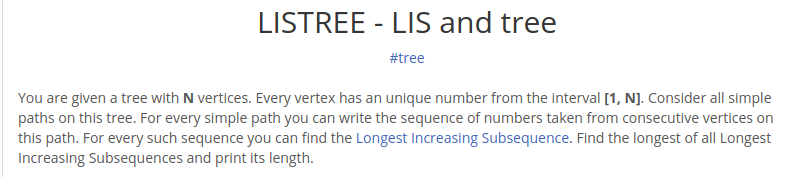
\includegraphics[scale=0.39]{assets/images/deskripsi.png}}
	\caption{Deskripsi soal \textit{LIS and TREE} pada situs penilaian daring SPOJ}
	\label{figure:deskripsi}
\end{figure}
\quad Di dalam soal tersebut dideskripsikan terdapat sebuah \textit{tree} dengan $N$ \textit{node}. Di mana setiap \textit{node} memiliki angka yang unik, dengan interval $1$ sampai $N$. Dalam soal ini di deskripsikan bahwa setiap \textit{path} merupakan \textit{simple path}, yang memiliki arti bahwa tidak ada \textit{node} yang berulang. Untuk setiap \textit{path} dapat dituliskan serangkaian angka yang diambil secara berurutan dari setiap \textit{node}. Untuk setiap rangkaian tersebut dapat dicari LIS nya masing-masing. Tujuan dari soal ini adalah untuk menemukan LIS terpanjang dari semua LIS yang terbentuk dari setiap \textit{path}.

\quad Format masukan diawali dengan sebuah bilangan bulat $T$ dimana $T(1\leq T\leq 1000)$ yang menggambarkan banyaknya \textit{testcase} atau \textit{data sets}. Kemudian untuk setiap $T$ terdapat sebuah bilangan bulat $N$ dimana $N(1\leq N\leq 100000)$ yang merepresentasikan jumlah \textit{node} untuk setiap \textit{testcase} yang nantinya akan membentuk \textit{tree}. Setelah itu terdapat $N-1$ baris dimana terdapat dua bilangan bulat $a$ dan $b$ dimana $(1\leq a,b\leq N)$ yang menunjukkan terdapat sebuah \textit{edge} yang menghubungkan \textit{node} $a$ dan \textit{node} $b$.

\quad Format keluaran berupa sebuah bilangan bulat yang menunjukkan panjang dari LIS terpanjang di antara semua \textit{simple path}. Contoh format masukan dan keluaran dapat dilihat pada Gambar \ref{figure:i/o}. 

\begin{figure}[H]
	\centerline{ 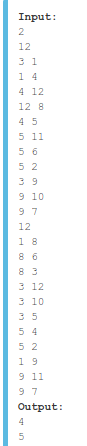
\includegraphics[scale=0.43]{assets/images/input-output.png}}
	\caption{Contoh format masukan pada situs penilaian daring SPOJ}
	\label{figure:i/o}
\end{figure}
\quad Dari contoh format masukkan pada Gambar \ref{figure:i/o} diminta jumlah kasus uji $(T)$ sebanyak $2$, kemudian pada kasus uji kedua diberi masukkan $12$ yang menggambarkan jumlah \textit{node} $(N)$. Kemudian terdapat $11$ baris yang berisikan dua bilangan bulat yaitu $a$ dan $b$, yang mengindikasikan bahwa kedua \textit{node} saling terhubung, dan \textit{node} $a$ menjadi \textit{parent} dari \textit{node} $b$, dimana pada akhirnya akan membentuk sebuah \textit{tree}. Proses pembentukkan tersebut dapat dilihat di Tabel \ref{tabel:visinput1}.
\begin{table}[H]
	\begin{tabular}{|p{0.5cm}|p{2.75cm}|p{3.0cm}|p{2.0cm}|}
		\hline
		No & Masukan $a$ dan $b$ & Bentuk Tree & Keterangan\\
		\hline
		1 & $a$ = 1 $b$ = 8 & \centering
		\begin{tikzpicture}
		[level/.style={sibling distance = 1.5cm/#1, level distance = 1.5cm}, scale=0.6,transform shape]
		\node[treenode]{1}
		child{
			node[treenode]{8}
		};
		\addvmargin{10mm}
		\end{tikzpicture} & Masukan baris ke-1
		\\ \hline
		2 & $a$ = 8 $b$ = 6 & \centering
		\begin{tikzpicture}
		[level/.style={sibling distance = 1.5cm/#1, level distance = 1.5cm}, scale=0.6,transform shape]
		\node[treenode]{1}
		child{
			node[treenode]{8}
			child{
				node[treenode]{6}
				}  
		};
		\addvmargin{10mm}
		\end{tikzpicture} & Masukan baris ke-2
		\\ \hline
		3 & $a$ = 8 $b$ = 3 & \centering
		\begin{tikzpicture}
		[level/.style={sibling distance = 2.5cm/#1, level distance = 1.5cm}, scale=0.6,transform shape]
		\node[treenode]{1}
		child{
			node[treenode]{8}
			child{
				node[treenode]{6}
			}
			child{
				node[treenode]{3}
				}
		};
		\addvmargin{10mm}
		\end{tikzpicture} & Masukan baris ke-3
		\\ \hline
	\end{tabular}\caption{Visualisasi proses pembentukkan \textit{tree} dari masukan pada daring. \label{tabel:visinput1}}
\end{table}

\quad Proses berlanjut hingga masukan terakhir, hingga membentuk \textit{tree} seperti pada Gambar \ref{fig:fulvis}.

\begin{figure}[H]
\centering
\begin{tikzpicture}[level/.style={sibling distance = 5cm/#1, level distance = 1.5cm}, scale=0.68,transform shape]
	\node[treenode]{1}
	child{
		node[treenode]{8}
		child{
			node[treenode]{6}
		}
		child{
			node[treenode]{3}
			child{
				node[treenode]{12}
				}
			child{
				node[treenode]{10}
			}
			child{
				node[treenode]{5}
				child{
					node[treenode]{4}
					}
				child{
					node[treenode]{2}
				}
			}	
		}
	}
	child{
		node[treenode]{9}
		child{
			node[treenode]{11}
			}
		child{
			node[treenode]{7}
		}	
	};
\end{tikzpicture}
\caption{Bentuk akhir tree sesuai masukan ke-2 pada contoh masukan\label{fig:fulvis}}
\end{figure}
\quad Dari contoh masukan kedua di situs penilaian daring SPOJ menunjukkan keluaran LIS yaitu 5, visualisasi untuk jawaban tersebut bisa dilihat di Gambar \ref{fig:ansvis}.
\begin{figure}[H]
	\centering
	\begin{tikzpicture}[level/.style={sibling distance = 5cm/#1, level distance = 1.5cm}, scale=0.68,transform shape]
	\node[treenode]{1}
	child{
		node[treenode,fill=green]{8}
		child{
			node[treenode]{6}
		}
		child{
			node[treenode,fill=green]{3}
			child{
				node[treenode]{12}
			}
			child{
				node[treenode]{10}
			}
			child{
				node[treenode]{5}
				child{
					node[treenode]{4}
				}
				child{
					node[treenode,fill=green]{2}
				}
			}	
		}
	}
	child{
		node[treenode,fill=green]{9}
		child{
			node[treenode,fill=green]{11}
		}
		child{
			node[treenode]{7}
		}	
	};
	\end{tikzpicture}
	\caption{\textit{Vertex} dengan warna hijau menunjukkan LIS dari contoh masukan kedua dari situs penilaian daring SPOJ\label{fig:ansvis}}
\end{figure}

\quad Beberapa batasan yang terdapat pada permasalahan \textit{LIS and TREE} adalah sebagai berikut:
\begin{enumerate}
	\item Besar ukuran berkas masukkan dalam sekali uji maksimal 2 MB.
	\item $(1\leq T\leq 1000)$.
	\item $N(1\leq N\leq 100000)$
	\item $(1\leq a,b\leq N)$
	\item Kombinasi dari node a dan b haruslah unik.
	\item Batas memori: 1536MB
	\item Batas sumber kode 50000B
	\item Batas waktu $ 2 $ detik.	
\end{enumerate}


\section{\quad Penyelesaian Permasalahan \textit{LIS and TREE} pada SPOJ}
\quad Pada subbab ini akan dijelaskan bagaimana menyelesaikan permasalahan \textit{LIS and TREE} dengan penjelasan permasalahan seperti pada subbab sebelumnya.

\quad Sesuai pada deskripsi masalah, dapat diketahui bahwa setiap \textit{node} memiliki \textit{parent} yang telah ditentukan sesuai dengan masukan, sesuai dengan penjelasan pada subbab 2.8.

\quad Untuk mengatasi hal tersebut maka digunakanlah konsep \textit{Disjoint set union} dengan menggunakan \textit{array} $2$ dimensi, sebagai contoh akan digunakan masukan seperti pada Gambar \ref{figure:custominput}.
\begin{figure}[H]
	\centerline{ 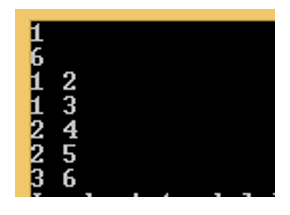
\includegraphics[scale=0.39]{assets/images/Input_contoh.PNG}}
	\caption{Contoh masukan yang digunakan.}
	\label{figure:custominput}
\end{figure}
\quad Visualisasi memasukan masukan pada contoh ke \textit{array} divisualisasikan pada Gambar \ref{figure:olahinput}.
\begin{figure}[H]
	\centerline{ 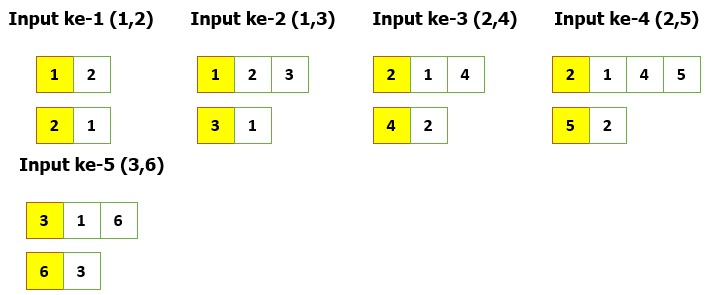
\includegraphics[scale=0.39]{assets/images/Olah_input.PNG}}
	\caption{Visualisasi pengolahan masukan}
	\label{figure:olahinput}
\end{figure}

\quad Dari pengolahan masukan tersebut terlihat bahwa elemen pertama untuk setiap \textit{array} menandakan sebagai \textit{parent} dari \textit{node} tersebut, kecuali untuk \textit{node} $1$ hal ini disebabkan \textit{node} tersebut akan menjadi \textit{root}. Maka dapat terbentuklah \textit{tree} seperti pada Gambar \ref{figure:treeinput}. 
\begin{figure}[H]
	\centerline{ 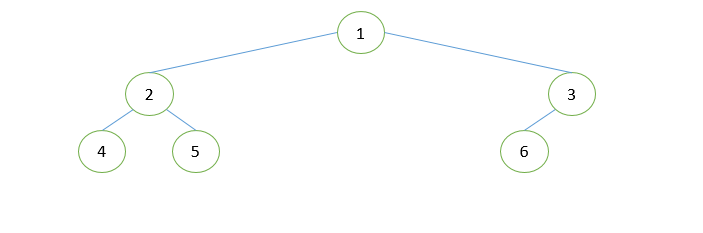
\includegraphics[scale=0.39]{assets/images/Tree_input.PNG}}
	\caption{Visualisasi bentuk \textit{tree} dari contoh masukan}
	\label{figure:treeinput}
\end{figure}
\quad Dalam persoalan \textit{LIS and TREE} LIS yang dicari merupakan sebuah \textit{path} dari \textit{tree} itu sendiri, dan \textit{path} ini merupakan sebuah \textit{simple path} seperti yang telah dijelaskan pada subbab 2.7. Maka untuk mendapatkan nilai LIS tersebut, secara umum terdapat beberapa \textit{case} agar mendapatkan nilai LIS dari setiap \textit{path} yang ada.

\quad \textit{Case} yang ada adalah sebagai berikut:
\begin{enumerate}
	\item \textit{Case} yang pertama adalah jika nilai \textit{node} yang lebih besar berada di atas \textit{node} tersebut, seperti pada Gambar \ref{fig:case1}. Menunjukkan bahwa nilai \textit{node} $a$ > $b$, sehingga arah \textit{path} dari bawah menuju ke atas.
	\item \textit{Case} yang kedua adalah jika nilai \textit{node} yang lebih besar berada di bawah \textit{node} tersebut, seperti pada Gambar \ref{fig:case2}. Menunjukkan bahwa nilai \textit{node} $a$ < $b$, sehingga arah \textit{path} dari atas menuju ke bawah.
	\item \textit{Case} yang kedua adalah jika nilai \textit{node} yang lebih besar berada di \textit{depth} yang sama dari \textit{node} tersebut, seperti pada Gambar \ref{fig:case3}. Menunjukkan bahwa nilai \textit{node} $a$ > $b$, sehingga arah \textit{path} dari bawah menuju ke atas kemudian menuju ke bawah.
\end{enumerate} 
\begin{figure}[H]
	\centering
	\begin{tikzpicture}
		[level/.style={sibling distance = 5cm/#1, level distance = 1.5cm}, scale=0.68,transform shape]
		\node[treenode,fill=green]{a}
		child{
			node[treenode]{}
			child{
				node[treenode]{}
				}
			child{
				node[treenode,fill=green]{b}
				}	
			}
		child{
			node[treenode]{}
			child{
				node[treenode]{}
				}
			child{
				node[treenode]{}
				}
			};
	\end{tikzpicture}\caption{Visualisasi \textit{case} ketika nilai \textit{node child \textgreater parent}.\label{fig:case1}}
\end{figure}
\begin{figure}[H]
	\centering
	\begin{tikzpicture}
	[level/.style={sibling distance = 5cm/#1, level distance = 1.5cm}, scale=0.68,transform shape]
	\node[treenode,fill=green]{a}
	child{
		node[treenode]{}
		child{
			node[treenode,fill=green]{b}
		}
		child{
			node[treenode]{}
		}	
	}
	child{
		node[treenode]{}
		child{
			node[treenode]{}
		}
		child{
			node[treenode]{}
		}
	};
	\end{tikzpicture}\caption{Visualisasi \textit{case} ketika nilai \textit{node parent \textgreater child.}\label{fig:case2}}
\end{figure}
\begin{figure}[H]
	\centering
	\begin{tikzpicture}
	[level/.style={sibling distance = 5cm/#1, level distance = 1.5cm}, scale=0.68,transform shape]
	\node[treenode]{}
	child{
		node[treenode]{}
		child{
			node[treenode,fill=green]{a}
		}
		child{
			node[treenode]{}
		}	
	}
	child{
		node[treenode]{}
		child{
			node[treenode]{}
		}
		child{
			node[treenode,fill=green]{b}
		}
	};
	\end{tikzpicture}\caption{Visualisasi \textit{case} ketika nilai \textit{node} yang lebih besar merupakan \textit{sibling}\label{fig:case3}}
\end{figure}

\quad Untuk dapat menyimpan hasil LIS dari setiap \textit{path} maka diperlukan dua \textit{segment tree} yang akan menyimpan nilai dari tiap interval. \textit{Segment tree} pertama akan menyimpan nilai LIS itu sendiri dan yang kedua akan menyimpan nilai LDS (Longest Decreasing Subsequence) kemudian nantinya jawaban akhir merupakan hasil perbandingan nilai dari dua \textit{segment tree} tersebut.
 
\quad Secara umum algoritma penyelesaian yang dilakukan untuk setiap \textit{node} adalah sebagai berikut:
\begin{enumerate}
	\item Tentukan \textit{child} yang menjadi \textit{big child} atau \textit{small child} menggunakan konsep \textit{Heavy-light Decomposition}.
	\item Lakukan rekursi ke \textit{small child}
	\item Lakukan perulangan untuk mencari LIS dan LDS dari \textit{parent} pada seluruh \textit{child} yang bukan merupakan \textit{bigchild}.
	\item Simpan hasil LIS dan LDS tersebut ke \textit{Segment Tree}.
	\item Cari nilai LIS dan LDS dari \textit{child} ke \textit{parent}.
	\item Simpan hasil LIS dan LDS tersebut ke \textit{Segment Tree}.
	\item Setelah selesai, kembalikan \textit{Segment Tree} ke kondisi semula.
	\item Lakukan rekursi ke \textit{big child}.
	\item Ulangi proses ke 3 hingga 6.
	\item Setelah selesai, biarkan kondisi \textit{Segment Tree} karena akan digunakan kembali.
	\item Lakukan proses hingga semua \textit{node} terlewati.
\end{enumerate}
\quad Proses diawali dari \textit{root} yaitu melakukan pengecekan \textit{child} mana yang merupakan \textit{big} atau \textit{small child} seperti pada Gambar \ref{fig:subproses1}, \ref{fig:subproses2}, dan \ref{fig:subproses3}.
\begin{figure}[H]
	\begin{subfigure}{.5\textwidth}
		\centering
		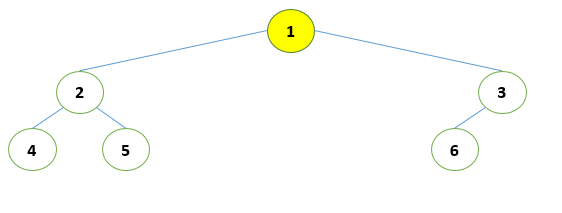
\includegraphics[scale=0.36]{assets/images/Ilustrasi_proses_1.PNG}
		\caption{Memeriksa \textit{child} dari root}
		\label{fig:subproses1}
	\end{subfigure}
	\begin{subfigure}{.5\textwidth}
		\centering
		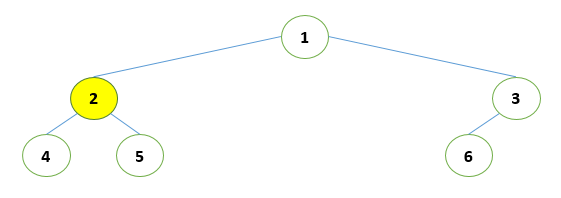
\includegraphics[scale=0.36]{assets/images/Ilustrasi_proses_2.PNG}
		\caption{\textit{Big child} dari \textit{root}}
		\label{fig:subproses2}
	\end{subfigure}
	\begin{subfigure}{.5\textwidth}
		\centering
		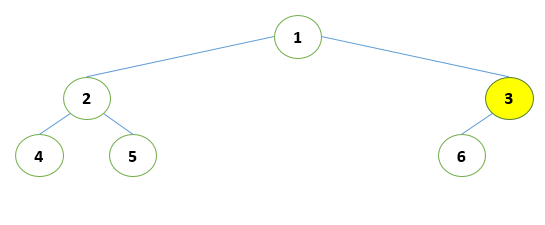
\includegraphics[scale=0.36]{assets/images/Ilustrasi_proses_3.PNG}
		\caption{\textit{Small child} dari \textit{root}}
		\label{fig:subproses3}
	\end{subfigure}
	\begin{subfigure}{.5\textwidth}
		\centering
		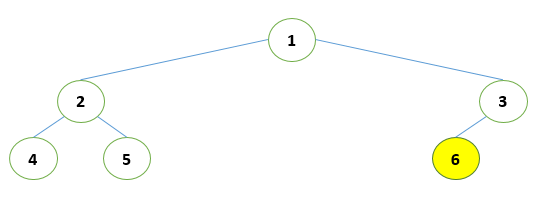
\includegraphics[scale=0.36]{assets/images/Ilustrasi_proses_4.PNG}
		\caption{\textit{Big child} dari \textit{node} 3}
		\label{fig:subproses4}
	\end{subfigure}
	\caption{Penentuan \textit{big child} dan \textit{small child} dari \textit{root}}
	\label{fig:proses1}
\end{figure}

\quad Dari proses sebelumnya diketahui bahwa \textit{small child} dari \textit{root} adalah \textit{node} 3, maka proses akan dilanjutkan pada \textit{node} 3. Pada \textit{node} tersebut dilakukan kembali pencari \textit{big} dan \textit{small child}. Karena hanya memiliki satu \textit{child} saja, maka proses akan langsung dilanjutkan pada \textit{big child}, yaitu \textit{node} 6, ditunjukkan oleh Gambar \ref{fig:subproses4}. 

\quad Pada \textit{node} 6 dilakukan pencarian LIS dan LDS seperti yang tertulis pada algoritma penyelesaian sebelumnya, pada Gambar \ref{fig:proses2} hingga \ref{fig:subproses13} dilakukan proses \textit{$query()$} untuk mencari LIS pada \textit{segment tree} dari rentang $1$ hingga $5$. Proses yang terjadi seperti yang telah dijelaskan pada subbab 2.4.
\begin{figure}[H]
	\vspace{-1.2cm}
	\begin{subfigure}{1.0\textwidth}
		\centering
		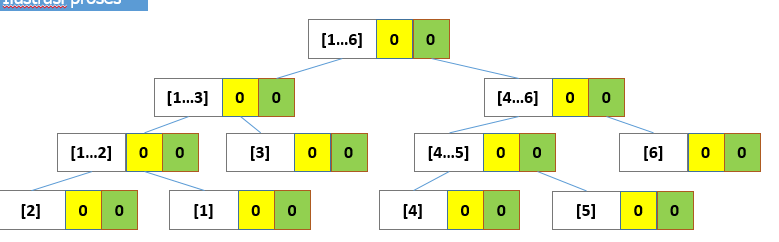
\includegraphics[scale=0.32]{assets/images/Ilustrasi_proses_5.PNG}
		\caption{Kondisi awal \textit{segment tree}}
		\label{fig:subproses5}
	\end{subfigure}
	\begin{subfigure}{1.0\textwidth}
		\centering
		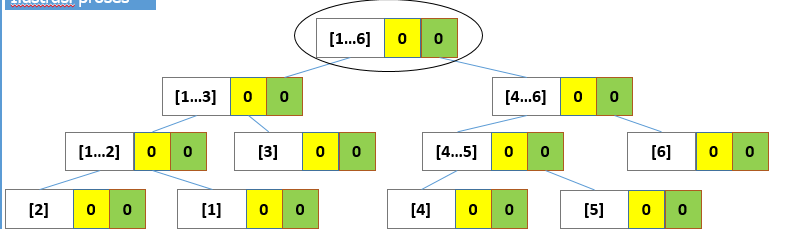
\includegraphics[scale=0.32]{assets/images/Ilustrasi_proses_6.PNG}
		\caption{Memeriksa rentang 1 hingga 6}
		\label{fig:subproses6}
	\end{subfigure}
	\begin{subfigure}{1.0\textwidth}
		\centering
		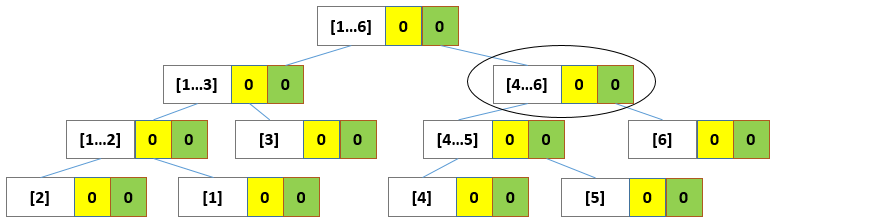
\includegraphics[scale=0.32]{assets/images/Ilustrasi_proses_7.PNG}
		\caption{Memeriksa rentang 4 hingga 6}
		\label{fig:subproses7}
	\end{subfigure}
	\begin{subfigure}{1.0\textwidth}
		\centering
		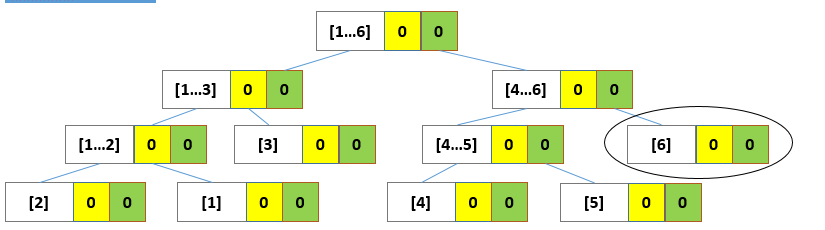
\includegraphics[scale=0.32]{assets/images/Ilustrasi_proses_8.PNG}
		\caption{\textit{Out of range}}
		\label{fig:subproses8}
	\end{subfigure}
	\begin{subfigure}{1.0\textwidth}
		\centering
		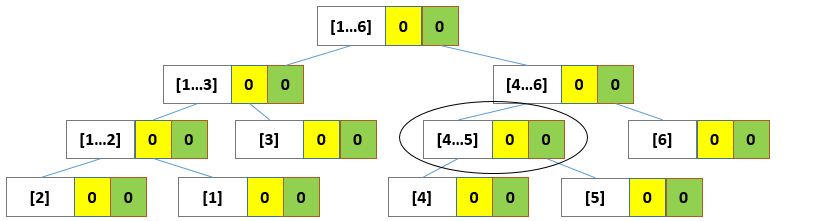
\includegraphics[scale=0.32]{assets/images/Ilustrasi_proses_9.PNG}
		\caption{Mengambil nilai rentang 4 hingga 5}
		\label{fig:subproses9}
	\end{subfigure}
	\begin{subfigure}{1.0\textwidth}
		\centering
		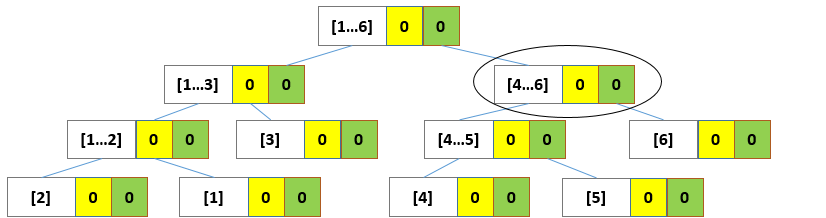
\includegraphics[scale=0.32]{assets/images/Ilustrasi_proses_10.PNG}
		\caption{Mengembalikan nilai ke atas}
		\label{fig:subproses10}
	\end{subfigure}
	\caption{Proses \textit{$query$} nilai LIS \textit{node} 6 pada \textit{right child} dari \textit{segment tree}}
	\label{fig:proses2}
\end{figure}
\begin{figure}[H]
	\begin{subfigure}{1.0\textwidth}
		\centering
		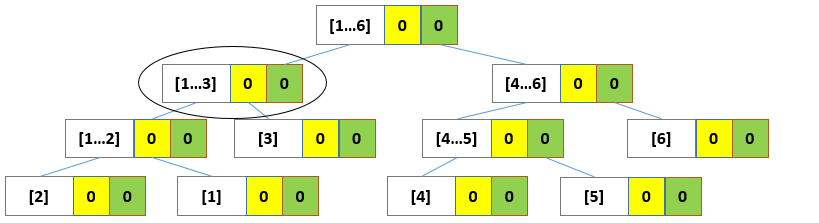
\includegraphics[scale=0.33]{assets/images/Ilustrasi_proses_11.PNG}
		\caption{Mengambil nilai rentang 1 hingga 3}
		\label{fig:subproses11}
	\end{subfigure}
	\begin{subfigure}{1.0\textwidth}
		\centering
		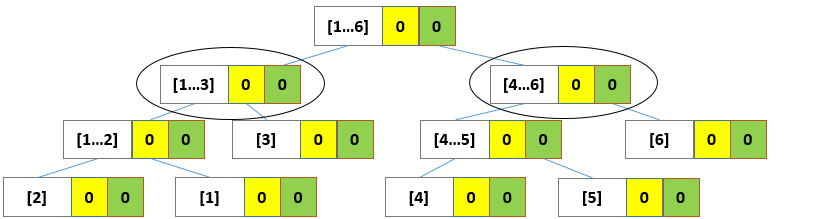
\includegraphics[scale=0.33]{assets/images/Ilustrasi_proses_12.PNG}
		\caption{Membandingkan nilai dengan \textit{sibling}}
		\label{fig:subproses12}
	\end{subfigure}
	\begin{subfigure}{1.0\textwidth}
		\centering
		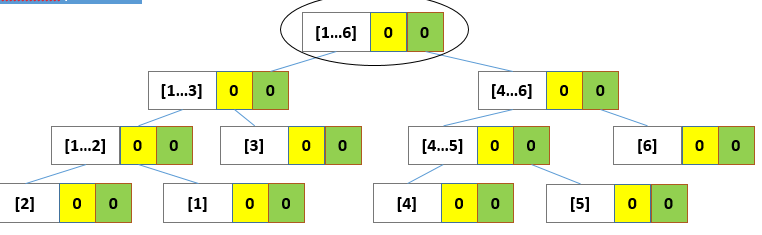
\includegraphics[scale=0.33]{assets/images/Ilustrasi_proses_13.PNG}
		\caption{Mengembalikan nilai ke \textit{root}}
		\label{fig:subproses13}
	\end{subfigure}
	\begin{subfigure}{1.0\textwidth}
		\centering
		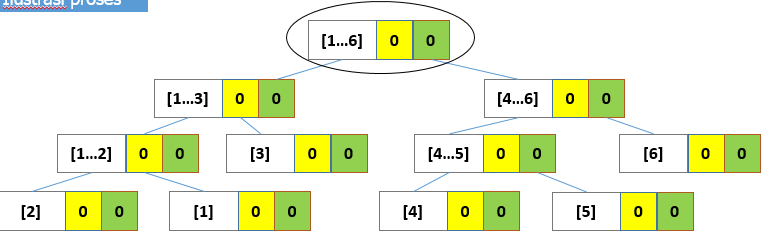
\includegraphics[scale=0.33]{assets/images/Ilustrasi_proses_14.PNG}
		\caption{\textit{Out of range}}
		\label{fig:subproses14}
	\end{subfigure}
	\caption{Proses \textit{$query$} nilai LIS \textit{node} 6 pada \textit{left child} dari \textit{segment tree} dan pengembalian nilai ke \textit{root}}
\end{figure}
\quad Pada Gambar \ref{fig:subproses14} dilakukan pencarian LDS untuk \textit{node} 6, dengan melakukan \textit{$query()$} rentang 7 pada \textit{segment tree}, karena hanya tersedia hingga rentang 6 maka langsung mengembalikan nilai.\newpage

\quad Kemudian hasil \textit{$query()$} disimpan pada variabel sementara milik \textit{node} 6, terlihat pada Gambar \ref{fig:subproses15} nilai LIS dan LDS sementara adalah $1$, maka hasil sementara saat ini adalah $1$.
\begin{figure}[H]
	\begin{subfigure}{1.0\textwidth}
		\centering
		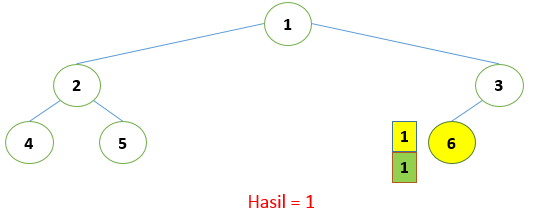
\includegraphics[scale=0.33]{assets/images/Ilustrasi_proses_15.PNG}
		\caption{Kondisi setelah proses \textit{$query$ node} 6}
		\label{fig:subproses15}
	\end{subfigure}
	\begin{subfigure}{1.0\textwidth}
		\centering
		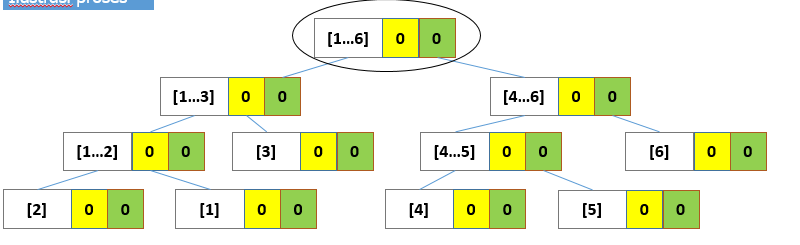
\includegraphics[scale=0.33]{assets/images/Ilustrasi_proses_16.PNG}
		\caption{Memeriksa \textit{root}}
		\label{fig:subproses16}
	\end{subfigure}
	\begin{subfigure}{1.0\textwidth}
		\centering
		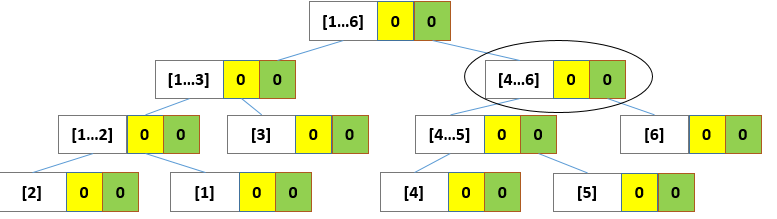
\includegraphics[scale=0.33]{assets/images/Ilustrasi_proses_17.PNG}
		\caption{Memeriksa rentang 4 hingga 6}
		\label{fig:subproses17}
	\end{subfigure}
	\begin{subfigure}{1.0\textwidth}
		\centering
		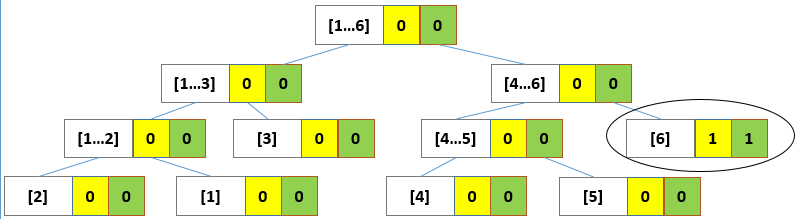
\includegraphics[scale=0.33]{assets/images/Ilustrasi_proses_18.PNG}
		\caption{Memperbarui nilai rentang 6}
		\label{fig:subproses18}
	\end{subfigure}
	\caption{Penyimpanan nilai untuk LIS dan LDS \textit{node} 6 dan \textit{$update()$} pada \textit{segment tree}}
	\label{fig:proses4}
\end{figure}\newpage
\quad Dikarenakan \textit{node} 6 merupakan \textit{big child} maka perlu dilakukan \textit{$update()$} pada \textit{segment tree}, \textit{update} akan dilakukan pada \textit{node} yang menyimpan nilai dari rentang 6. Proses fungsi \textit{$update()$} sendiri seperti yang telah dijelaskan pada subbab 2.4. Gambar \ref{fig:subproses16} hingga Gambar \ref{fig:subproses20}.
\begin{figure}[H]
	\begin{subfigure}{1.0\textwidth}
		\centering
		\includegraphics[scale=0.33]{assets/images/Ilustrasi_proses_19.PNG}
		\caption{Mengembalikan nilai ke atas}
		\label{fig:subproses19}
	\end{subfigure}
	\begin{subfigure}{1.0\textwidth}
		\centering
		\includegraphics[scale=0.33]{assets/images/Ilustrasi_proses_20.PNG}
		\caption{Mengembalikan nilai ke \textit{root}}
		\label{fig:subproses20}
	\end{subfigure}
	\begin{subfigure}{1.0\textwidth}
		\centering
		\includegraphics[scale=0.33]{assets/images/Ilustrasi_proses_21.PNG}
		\caption{Melanjutkan proses ke \textit{node} 3}
		\label{fig:subproses21}
	\end{subfigure}
	\caption{Proses \textit{$update()$} pada \textit{segment tree} dan rekursi ke \textit{parent}}
	\label{fig:proses5}
\end{figure}

\quad Proses dilanjutkan ke \textit{parent} dari \textit{node} 6, yaitu \textit{node} 3, divisualkan pada Gambar \ref{fig:subproses21}. Proses yang dilakukan sama yaitu menjalankan \textit{$query()$} untuk mencari nilai LIS dan LDS pada \textit{segment tree}. Nilai yang didapatkan adalah 2 untuk LIS dan LDS, yang disimpan pada variabel sementara milik \textit{node} 3 seperti pada Gambar \ref{fig:subproses22}.
\begin{figure}[H]
	\begin{subfigure}{1.0\textwidth}
		\centering
		\includegraphics[scale=0.33]{assets/images/Ilustrasi_proses_22.PNG}
		\caption{Kondisi setelah memproses \textit{node} 3}
		\label{fig:subproses22}
	\end{subfigure}
	\begin{subfigure}{1.0\textwidth}
		\centering
		\includegraphics[scale=0.33]{assets/images/Ilustrasi_proses_23.PNG}
		\caption{Kondisi \textit{segment tree} seperti semula}
		\label{fig:subproses23}
	\end{subfigure}
	\begin{subfigure}{1.0\textwidth}
		\centering
		\includegraphics[scale=0.33]{assets/images/Ilustrasi_proses_24.PNG}
		\caption{Kondisi setelah selesai memproses \textit{node} 4 dan 5}
		\label{fig:subproses24}
	\end{subfigure}
	\caption{Pengembalian kondisi \textit{segment tree} seperti semula}
	\label{fig:proses6}
\end{figure}

\quad Karena \textit{node} 3 merupakan \textit{small child}, maka sebelum kembali ke \textit{parent}nya, kondisi \textit{segment tree} perlu dikembalikan seperti semula, yaitu menjadikan seluruh nilai yang ada didalamnya menjadi $0$. Seperti pada Gambar \ref{fig:subproses23}.

\quad Proses dilanjutkan ke \textit{big child} dari \textit{root} yaitu \textit{node} 2 seperti pada Gambar \ref{fig:subproses24}. Tahapan yang dilakukan sama seperti pada \textit{node} 3, dengan mencari \textit{big child} dan \textit{small child} kemudian menyimpan nilai pada variabel sementara untuk setiap \textit{node}. Setelah selesai memproses seluruh \textit{child} dilakukan \textit{query} untuk LIS dan LDS pada \textit{node} 2, dari kondisi \textit{segment tree} seperti pada Gambar \ref{fig:subproses25}, dan akan menyimpan hasilnya pada variabel sementara \textit{node} 2, seperti pada Gambar \ref{fig:subproses26}. Kondisi akhir dari keseluruhan proses ditunjukan oleh Gambar \ref{fig:subproses27} dengan keluaran akhir yaitu $3$.
\begin{figure}[H]
	\begin{subfigure}{1.0\textwidth}
		\centering
		\includegraphics[scale=0.39]{assets/images/Ilustrasi_proses_25.PNG}
		\caption{Kondisi \textit{segment tree} pada \textit{node} 2}
		\label{fig:subproses25}
	\end{subfigure}
	\begin{subfigure}{1.0\textwidth}
		\centering
		\includegraphics[scale=0.39]{assets/images/Ilustrasi_proses_26.PNG}
		\caption{Kondisi setelah proses pada \textit{node} 2}
		\label{fig:subproses26}
	\end{subfigure}
	\begin{subfigure}{1.0\textwidth}
		\centering
		\includegraphics[scale=0.39]{assets/images/Ilustrasi_proses_27.PNG}
		\caption{Kondisi akhir dari keseluruhan proses}
		\label{fig:subproses27}
	\end{subfigure}
	\caption{Proses pencarian LIS dan LDS pada \textit{big child} dari \textit{root} dan pada \textit{root}}
	\label{fig:proses7}
\end{figure}	
	\chapter{DESAIN}
\label{chapter:desain}

Pada bab ini akan dibahas tentang desain dan algoritma untuk menyelesaikan permasalahan pada Tugas Akhir ini.

\section{\quad Desain Penyelesaian Permasalahan \textit{LIS and TREE by value}}
\quad Pada subbab ini akan dijelaskan desain penyelesaian permasalahan \textit{LIS and TREE} dengan pendekatan \textit{Segment Tree}.
	\subsection{\quad Definisi Umum Sistem}
	\quad Sistem akan menerima masukan berupa sebuah bilangan bulat $T$ yang mewakili banyaknya kasus uji. Selanjutnya sistem menerima masukan sebuah bilangan bulat $n$ yang mewakili jumlah \textit{node} untuk kasus uji tersebut. Kemudian sistem akan menerima masukan berupa dua buah bilangan bulat $a$ dan $b$ yang merepresentasikan nilai dan hubungan antar \textit{node} seperti yang telah dijelaskan pada subbab 2.6. Kemudian sistem akan menggambarkan masukkan tersebut sebagai sebuah \textit{tree} dengan memanggil fungsi \textit{init} setelah \textit{tree} terbentuk akan melakukan pencarian LIS yang akan memenuhi persoalan tersebut, yang pada akhirnya akan menjadi keluaran akhir dari program. Pseudocode fungsi \textit{main} ditunjukkan oleh Gambar \ref{figure:fungsi_main}.
	
	\quad Pada fungsi \textit{main} terdapat variabel $T$ yang merupakan jumlah kasus uji dan $n$ yang merupakan jumlah \textit{node}. Setiap akan menerima masukan baru, fungsi \textit{main} akan mengosongkan terlebih dahulu isi daripada masukan yang sebelumnya, dilakukan dengan menggunakan fungsi \textit{clear} (baris ke 5). Kemudian fungsi akan memasukkan \textit{push} (baris ke 8 dan 9) nilai masukan yang baru. Lalu akan dipanggil fungsi \textit{init} dan \textit{dfs} yang akan dijelaskan pada subbab berikutnya.
	\begin{figure}
		\vspace{-0.5cm}\centering
		\begin{tabular}{|p{3cm}|p{6cm}|}
			\hline
			\multicolumn{2}{|p{0.8\textwidth}|}{ %
				$\proc{Main}()$}\\ \hline
			\multicolumn{2}{|p{0.8\textwidth}|}{ %
				1 $\proc{\textbf{input}}\quad T$}\\
			\multicolumn{2}{|p{0.8\textwidth}|}{ %
				2 \While $T--$}\\
			\multicolumn{2}{|p{0.8\textwidth}|}{ %
				3 \quad $\proc{\textbf{input}}\quad N$}\\
			\multicolumn{2}{|p{0.8\textwidth}|}{ %
				4 \quad $\proc{\textbf{for}}\quad i \quad \gets \quad 1 \quad \proc{\textbf{to}\quad N}$}\\
			\multicolumn{2}{|p{0.8\textwidth}|}{ %
				5 \quad \quad $\proc{\textbf{Clear}(inp[i])}$}\\
			\multicolumn{2}{|p{0.8\textwidth}|}{ %
				6 \quad $\proc{\textbf{for}}\quad i \quad \gets \quad 1 \quad \proc{\textbf{to}\quad N-1}$}\\
			\multicolumn{2}{|p{0.8\textwidth}|}{ %
				7 \quad \quad $\proc{\textbf{input}}\quad a$}\\
			\multicolumn{2}{|p{0.8\textwidth}|}{ %
				8 \quad \quad $\proc{\textbf{input}}\quad b$}\\
			\multicolumn{2}{|p{0.8\textwidth}|}{ %
				9 \quad \quad $\proc{\textbf{Push}(inp[a],b)}$}\\
			\multicolumn{2}{|p{0.8\textwidth}|}{ %
				10 \quad \quad $\proc{\textbf{Push}(inp[a],b)}$}\\
			\multicolumn{2}{|p{0.8\textwidth}|}{ %
				11 \quad $\proc{ans} \quad \gets 0$}\\
			\multicolumn{2}{|p{0.8\textwidth}|}{ %
				12 \quad $\proc{cnt} \quad \gets 0$}\\
			\multicolumn{2}{|p{0.8\textwidth}|}{ %
				13 \quad $\proc{\textbf{init}(1,-1)}$}\\
			\multicolumn{2}{|p{0.8\textwidth}|}{ %
				14 \quad $\proc{\textbf{Dfs}(1,-1,0)}$}\\
			\multicolumn{2}{|p{0.8\textwidth}|}{ %
				15 \quad $\proc{\textbf{Output}\quad ans}$}\\
				\hline
		\end{tabular}
		\caption{\textit{Pseudocode} Fungsi Main \label{figure:fungsi_main}}
	\end{figure}	
	\subsection{\quad Desain Algoritma}
	\quad Sistem terdiri dari 4 fungsi utama, yaitu fungsi \textit{init}, \textit{dfs}, \textit{query}, \textit{update}. Pada subbab ini akan dijelaskan desain algoritma keempat fungsi tersebut.
	\subsubsection{\quad Desain Fungsi \textit{init}}
	\quad Fungsi \textit{init} digunakan untuk membentuk \textit{tree} dari masukan pada fungsi \textit{main}, ditunjukkan oleh Gambar \ref{figure:fungsi_init}. Variabel $now$ merepresentasikan nilai \textit{node} saat ini, dan $parent$ merepresentasikan nilai \textit{node} yang menjadi \textit{parent} dari \textit{node} saat ini. Pada fungsi ini dilakukan iterasi untuk mendapatkan total jumlah \textit{child} dari keseluruhan \textit{tree} untuk setiap \textit{node} dan dilakukan \textit{preorder numbering} yang diwakili oleh variabel $in[]$ dan $out[]$.
	\begin{figure}
		\vspace{-0.5cm}\centering
		\begin{tabular}{|p{3cm}|p{6cm}|}
			\hline
			\multicolumn{2}{|p{0.8\textwidth}|}{ %
				$\proc{init(now,parent)}$}\\ \hline
			\multicolumn{2}{|p{0.8\textwidth}|}{ %
				1 $\proc{size[now]\quad}\gets1$}\\
			\multicolumn{2}{|p{0.8\textwidth}|}{ %
				2 $\proc{in[now]\quad}\gets++cnt$}\\
			\multicolumn{2}{|p{0.8\textwidth}|}{ %
				3 $\proc{num[cnt]\quad}\gets now$}\\
			\multicolumn{2}{|p{0.8\textwidth}|}{ %
				4 $\proc{\textbf{for}}\quad i \quad \gets \quad 0 \quad \proc{\textbf{to}\quad Sizeof(inp[now]-1)}$}\\
			\multicolumn{2}{|p{0.8\textwidth}|}{ %
				5 \quad \If $\proc{inp[now][i]}\gets parent\quad\proc{\textbf{continue}}$}\\
			\multicolumn{2}{|p{0.8\textwidth}|}{ %
				6 \quad $\proc{\textbf{init}(inp[now][i],now)}$}\\
			\multicolumn{2}{|p{0.8\textwidth}|}{ %
				7 \quad $\proc{size[now]}\quad\gets\proc{size[now]\quad+\quad size[inp[now][i]}$}\\
			\multicolumn{2}{|p{0.8\textwidth}|}{ %
				8 $\proc{out[now]}\quad\gets\proc{cnt}$}\\
			\hline
		\end{tabular}
		\caption{\textit{Pseudocode} Fungsi init \label{figure:fungsi_init}}
	\end{figure}
	\subsubsection{\quad Desain Fungsi \textit{Dfs}}
	\quad Fungsi DFS merupakan fungsi utama untuk menemukan LIS dari \textit{path} yang ada ditunjukkan oleh Gambar \ref{figure:fungsi_dfs}. Parameter variabel yang dibutuhkan adalah $now$ sebagai representasi nilai \textit{node} saat ini, $parent$ sebagai representasi nilai dari \textit{parent} untuk \textit{node} saat ini, dan $flag$ sebagai variabel penanda apakah \textit{node} tersebut merupakan \textit{bigchild} atau \textit{smallchild}. Di awal fungsi (baris kode 1-5) dilakukan penentuan \textit{node} mana yang menjadi \textit{big child} atau \textit{small child}, hal ini ditentukan dengan cara membandingkan ukuran \textit{node} tersebut dengan \textit{sibling}nya. Kemudian fungsi akan melakukan rekursi ke \textit{node} yang menjadi \textit{smallchild} (baris kode 6-9) dan dilanjutkan rekursi ke \textit{node} yang menjadi \textit{bigchild} (baris kode 10-11). Setelah itu dilakukan perulangan untuk setiap \textit{child} dari \textit{node} kecuali \textit{bigchild} dalam perulangan ini dilakukan pencarian LIS dan LDS serta melakukan \textit{update} pada \textit{segment tree} untuk nilai LIS dan LDS di \textit{subtree} sebelumnya (baris kode 12-31). Lalu jika \textit{node} yang telah diproses merupakan \textit{smallchild} maka isi \textit{segment tree} akan di kembalikan seperti semula, jika tidak isi \textit{segment tree} akan dipertahankan (baris kode 32-36). Pada prosesnya fungsi \textit{dfs} juga memanggil fungsi lain yaitu $query$ dan $update$.
	 
	\quad Fungsi $query$ ditunjukkan oleh Gambar \ref{figure:fungsi_query}. Terdapat 6 variabel yang menjadi parameter untuk fungsi ini, $idx$ merepresentasikan posisi \textit{node} saat ini, $l$ dan $r$ merupakan representasi rentang index yang diwakili oleh \textit{node} saat ini, $x$ dan $y$ merupakan representasi rentang index yang akan diambil nilainya, $flag$ merupakan penanda apakah harus mengambil nilai di \textit{segment tree} yang berisikan LIS atau LDS. Fungsi ini akan melakukan rekursi ke \textit{left child} kemudian dilanjutkan ke \textit{right child} hingga pada akhirnya mendapatkan nilai maksimal dari kedua rentang tersebut.
	 
	\quad Fungsi \textit{update} yang ditunjukkan oleh Gambar \ref{figure:fungsi_update}. Terdapat 6 variabel yang menjadi parameter untuk fungsi ini, $idx$ merepresentasikan posisi \textit{node} saat ini, $l$ dan $r$ merupakan representasi rentang index yang diwakili oleh \textit{node} saat ini, $x$ merupakan representasi index yang ingin di\textit{update}.
		\begin{figure}
			\vspace{-0.5cm}\centering
			\begin{tabular}{|p{9cm}|p{9cm}|}
				\hline
				\multicolumn{2}{|p{0.8\textwidth}|}{ %
					$\proc{Dfs}(now,parent,flag)$}\\ \hline
				\multicolumn{2}{|p{0.8\textwidth}|}{ %
					1 $\proc{\textbf{for}}\quad i \quad \gets \quad 0 \quad \proc{\textbf{to}\quad Sizeof(inp[now]-1)}$}\\
				\multicolumn{2}{|p{0.8\textwidth}|}{ %
					2 \quad \If \quad $\proc{temp}\quad\gets\proc{parent}\quad\proc{\textbf{continue}}$}\\
				\multicolumn{2}{|p{0.8\textwidth}|}{ %
					3 \quad \If $\proc{size[temp]}>maks$}\\
				\multicolumn{2}{|p{0.8\textwidth}|}{ %
					4 \quad \quad $\proc{maks}\quad\gets\quad\proc{size[temp]}$}\\
				\multicolumn{2}{|p{0.8\textwidth}|}{ %
					5 \quad \quad $\proc{bigchild}\quad\gets\quad\proc{temp}$}\\
				\multicolumn{2}{|p{0.8\textwidth}|}{ %
					6 $\proc{\textbf{for}}\quad i \quad \gets \quad 0 \quad \proc{\textbf{to}\quad Sizeof(inp[now]-1)}$}\\
				\multicolumn{2}{|p{0.8\textwidth}|}{ %
					7 \quad $\proc{temp}\quad\gets\quad\proc{inp[now][i]}$}\\
				\multicolumn{2}{|p{0.8\textwidth}|}{ %
					8 \quad \If $\proc{temp\quad!=\quad parent}\quad \textbf{and} \quad \proc{temp\quad!=\quad bigchild}$}\\
				\multicolumn{2}{|p{0.8\textwidth}|}{ %
					9 \quad \quad $\proc{\textbf{Dfs}(temp,now,0)}$}\\
				\multicolumn{2}{|p{0.8\textwidth}|}{ %
					10 \If $\proc{bigchild}\quad\gets\quad0$}\\
				\multicolumn{2}{|p{0.8\textwidth}|}{ %
					11 \quad $\proc{\textbf{Dfs}(big,now,1)}$}\\
				\multicolumn{2}{|p{0.8\textwidth}|}{ %
					12 $\proc{\textbf{for}}\quad i \quad \gets \quad 0 \quad \proc{\textbf{to}\quad Sizeof(inp[now]-1)}$}\\
				\multicolumn{2}{|p{0.8\textwidth}|}{ %
					13 \quad $\proc{temp}\quad\gets\quad\proc{inp[now][i]}$}\\
				\multicolumn{2}{|p{0.8\textwidth}|}{ %
					14 \quad \If $\proc{temp\quad=\quad parent}\quad \textbf{and} \quad \proc{temp\quad=\quad bigchild}$}\\
				\multicolumn{2}{|p{0.8\textwidth}|}{ %
					15 \quad \quad $\textbf{continue}$}\\
				\multicolumn{2}{|p{0.8\textwidth}|}{ %
					16 \quad $\proc{\textbf{foreach}\quad child\quad\textbf{in}\quad temp}$}\\
				\multicolumn{2}{|p{0.8\textwidth}|}{ %
					17 \quad \quad \If $\proc{child\quad<\quad now}$}\\
				\multicolumn{2}{|p{0.8\textwidth}|}{ %
					18 \quad \quad \quad 
					$\proc{maks=\textbf{query}(0,1,N,now+1,N,1)}$}\\
				\multicolumn{2}{|p{0.8\textwidth}|}{ %
					19 \quad \quad \quad $\proc{ans=\textbf{max}(ans,maks+1+dpUp[child])}$}\\
				\multicolumn{2}{|p{0.8\textwidth}|}{ %
					20 \quad \quad $\proc{\textbf{else}}$}\\
				\multicolumn{2}{|p{0.8\textwidth}|}{ %
					21 \quad \quad \quad $\proc{maks=\textbf{query}(0,1,N,1,now-1,0)}$}\\
				\multicolumn{2}{|p{0.8\textwidth}|}{ %
					22 \quad \quad \quad $\proc{ans=\textbf{max}(ans,maks+1+dpDec[child])}$}\\
				\multicolumn{2}{|p{0.8\textwidth}|}{ %
					23 \quad $\proc{maks=\textbf{query}(0,1,N,1,child-1,0)}$}\\
				\multicolumn{2}{|p{0.8\textwidth}|}{ %
					24 \quad $\proc{ans=\textbf{max}(ans,maks+1+dpDec[child])}$}\\
				\multicolumn{2}{|p{0.8\textwidth}|}{ %
					25 \quad $\proc{maks=\textbf{query}(0,1,N,child+1,N,1)}$}\\
				\multicolumn{2}{|p{0.8\textwidth}|}{ %
					26 \quad $\proc{ans=\textbf{max}(ans,maks+1+dpUp[child])}$}\\
				\multicolumn{2}{|p{0.8\textwidth}|}{ %
					27 \quad $\proc{\textbf{foreach}\quad child\quad\textbf{in}\quad temp}$}\\
				\multicolumn{2}{|p{0.8\textwidth}|}{ %
					28 \quad \quad $\proc{\textbf{update}(0,1,N,child,dpUp[child],dpDec[child])}$}\\
				\multicolumn{2}{|p{0.8\textwidth}|}{ %
					29 $\proc{dpUp[now]=\textbf{query}(0,1,N,1,now-1,0)+1}$}\\
				\multicolumn{2}{|p{0.8\textwidth}|}{ %
					30 $\proc{dpDec[now]=\textbf{query}(0,1,N,now+1,N,1)+1}$}\\
				\multicolumn{2}{|p{0.8\textwidth}|}{ %
					31 $\proc{ans=\textbf{max}(ans,\textbf{max}(dpUp[now],dpDec[now]))}$}\\
				\multicolumn{2}{|p{0.8\textwidth}|}{ %
					32 \If $\proc{flag\quad=\quad0}$}\\
				\multicolumn{2}{|p{0.8\textwidth}|}{ %
					33 \quad $\proc{\textbf{foreach}\quad child\quad\textbf{in}\quad now}$}\\
				\multicolumn{2}{|p{0.8\textwidth}|}{ %
					34 \quad \quad $\proc{\textbf{update}(0,1,N,child,0,0)}$}\\
				\multicolumn{2}{|p{0.8\textwidth}|}{ %
					35 $\proc{\textbf{else}}$}\\
				\multicolumn{2}{|p{0.8\textwidth}|}{ %
					36 \quad $\proc{\textbf{update}(0,1,N,now,dpUp[now],dpDec[now])}$}\\
				\hline
			\end{tabular}
			\caption{\textit{Pseudocode} Fungsi Dfs \label{figure:fungsi_dfs}}
		\end{figure}
	\begin{figure}
		\vspace{-0.5cm}\centering
		\begin{tabular}{|p{3cm}|p{6cm}|}
			\hline
			\multicolumn{2}{|p{0.8\textwidth}|}{ %
				$\proc{query(idx,l,r,x,y,flag)}$}\\ \hline
			\multicolumn{2}{|p{0.8\textwidth}|}{ %
				1 \If $\proc{l > y or r < x}$}\\
			\multicolumn{2}{|p{0.8\textwidth}|}{ %
				2 \quad $\proc{\textbf{return} 0}$}\\
			\multicolumn{2}{|p{0.8\textwidth}|}{ %
				3 \If $\proc{x <= l and r <= y}$}\\
			\multicolumn{2}{|p{0.8\textwidth}|}{ %
				4 \quad \If $\proc{flag = 0}$}\\
			\multicolumn{2}{|p{0.8\textwidth}|}{ %
				5 \quad \quad $\proc{\textbf{return} inc[idx]}$}\\
			\multicolumn{2}{|p{0.8\textwidth}|}{ %
				6 \quad $\proc{\textbf{else}}$}\\
			\multicolumn{2}{|p{0.8\textwidth}|}{ %
				7 \quad \quad $\proc{\textbf{return} dec[idx]}$}\\
			\multicolumn{2}{|p{0.8\textwidth}|}{ %
				8 $\proc{left = \textbf{query}((idx*2)+1,l,(l+r)/2,x,y,flag)}$}\\
			\multicolumn{2}{|p{0.8\textwidth}|}{ %
				9 $\proc{right = \textbf{query}((idx*2)+2,((l+r)/2)+1,r,x,y,flag)}$}\\
			\multicolumn{2}{|p{0.8\textwidth}|}{ %
				10 $\proc{\textbf{return max}(left,right)}$}\\
			\hline
		\end{tabular}
		\caption{\textit{Pseudocode} Fungsi query \label{figure:fungsi_query}}
	\end{figure}		 
	\begin{figure}
		\centering
		\begin{tabular}{|p{3cm}|p{6cm}|}
			\hline
			\multicolumn{2}{|p{0.8\textwidth}|}{ %
				$\proc{update(idx,l,r,x,a,b)}$}\\ \hline
			\multicolumn{2}{|p{0.8\textwidth}|}{ %
				1 \If $\proc{l = r}$}\\
			\multicolumn{2}{|p{0.8\textwidth}|}{ %
				2 \quad $\proc{inc[idx] = a}$}\\
			\multicolumn{2}{|p{0.8\textwidth}|}{ %
				3 \quad $\proc{dcr[idx] = b}$}\\
			\multicolumn{2}{|p{0.8\textwidth}|}{ %
				4 \quad $\proc{\textbf{return}}$}\\
			\multicolumn{2}{|p{0.8\textwidth}|}{ %
				5 \If $\proc{x <= (l+r)/2}$}\\
			\multicolumn{2}{|p{0.8\textwidth}|}{ %
				6 \quad $\proc{\textbf{update}((idx*2)+1,l,(l+r)/2,x,a,b)}$}\\
			\multicolumn{2}{|p{0.8\textwidth}|}{ %
				7 $\proc{\textbf{else}}$}\\
			\multicolumn{2}{|p{0.8\textwidth}|}{ %
				8 \quad $\proc{\textbf{update}((idx*2)+2,((l+r)/2)+1,r,x,a,b)}$}\\
			\multicolumn{2}{|p{0.8\textwidth}|}{ %
				9 $\proc{inc[idx] = \textbf{max}(inc[(idx*2)+1],inc[(idx*2)+2])}$}\\
			\multicolumn{2}{|p{0.8\textwidth}|}{ %
				10 $\proc{dcr[idx] = \textbf{max}(dcr[(idx*2)+1],dcr[(idx*2)+2])}$}\\
			\hline
		\end{tabular}
		\caption{\textit{Pseudocode} Fungsi update \label{figure:fungsi_update}}
	\end{figure}

	
\section{\quad Desain Penyelesaian Permasalahan \textit{LIS and TREE by reference}}
\quad Pada subbab ini akan dijelaskan desain penyelesaian permasalahan \textit{LIS and TREE} dengan pendekatan \textit{pointer}. 
	\subsection{\quad Definisi Umum Sistem}
	\quad Sistem akan menerima masukan berupa sebuah bilangan bulat $T$ yang mewakili banyaknya kasus uji. Selanjutnya sistem menerima masukan sebuah bilangan bulat $n$ yang mewakili jumlah \textit{node} untuk kasus uji tersebut. Kemudian sistem akan menerima masukan berupa dua buah bilangan bulat $a$ dan $b$ yang merepresentasikan nilai dan hubungan antar \textit{node} seperti yang telah dijelaskan pada subbab 2.6. Kemudian sistem akan menggambarkan masukkan tersebut sebagai sebuah \textit{tree} dengan memanggil fungsi \textit{init} setelah \textit{tree} terbentuk akan melakukan pencarian LIS yang akan memenuhi persoalan tersebut, yang pada akhirnya akan menjadi keluaran akhir dari program. Pseudocode fungsi \textit{main} ditunjukkan oleh Gambar \ref{figure:fungsi_main2}.
	
	\quad Pada fungsi \textit{main} terdapat variabel $T$ yang merupakan jumlah kasus uji dan $n$ yang merupakan jumlah \textit{node}. Setiap akan menerima masukan baru, fungsi \textit{main} akan mengosongkan terlebih dahulu isi daripada masukan yang sebelumnya, dilakukan dengan menggunakan fungsi \textit{clear} (baris ke 5). Kemudian fungsi akan memasukkan \textit{push} (baris ke 8 dan 9) nilai masukan yang baru. Lalu akan dipanggil fungsi \textit{init} dan \textit{dfs} yang akan dijelaskan pada subbab berikutnya.
	\begin{figure}
		\vspace{-0.5cm}\centering
		\begin{tabular}{|p{3cm}|p{6cm}|}
			\hline
			\multicolumn{2}{|p{0.8\textwidth}|}{ %
				$\proc{Main}()$}\\ \hline
			\multicolumn{2}{|p{0.8\textwidth}|}{ %
				1 $\proc{\textbf{input}}\quad T$}\\
			\multicolumn{2}{|p{0.8\textwidth}|}{ %
				2 \While $T--$}\\
			\multicolumn{2}{|p{0.8\textwidth}|}{ %
				3 \quad $\proc{\textbf{input}}\quad N$}\\
			\multicolumn{2}{|p{0.8\textwidth}|}{ %
				4 \quad $\proc{\textbf{for}}\quad i \quad \gets \quad 1 \quad \proc{\textbf{to}\quad N}$}\\
			\multicolumn{2}{|p{0.8\textwidth}|}{ %
				5 \quad \quad $\proc{\textbf{Clear}(inp[i])}$}\\
			\multicolumn{2}{|p{0.8\textwidth}|}{ %
				6 \quad $\proc{\textbf{for}}\quad i \quad \gets \quad 1 \quad \proc{\textbf{to}\quad N-1}$}\\
			\multicolumn{2}{|p{0.8\textwidth}|}{ %
				7 \quad \quad $\proc{\textbf{input}}\quad a$}\\
			\multicolumn{2}{|p{0.8\textwidth}|}{ %
				8 \quad \quad $\proc{\textbf{input}}\quad b$}\\
			\multicolumn{2}{|p{0.8\textwidth}|}{ %
				9 \quad \quad $\proc{\textbf{Push}(inp[a],b)}$}\\
			\multicolumn{2}{|p{0.8\textwidth}|}{ %
				10 \quad \quad $\proc{\textbf{Push}(inp[a],b)}$}\\
			\multicolumn{2}{|p{0.8\textwidth}|}{ %
				11 \quad $\proc{result} \quad \gets 0$}\\
			\multicolumn{2}{|p{0.8\textwidth}|}{ %
				12 \quad $\proc{\textbf{init}(1,-1)}$}\\
			\multicolumn{2}{|p{0.8\textwidth}|}{ %
				13 \quad $\proc{\textbf{Dfs}(1,-1,\text{\&}a,\text{\&}b)}$}\\
			\multicolumn{2}{|p{0.8\textwidth}|}{ %
				14 \quad $\proc{\textbf{Output}\quad result}$}\\
			\hline
		\end{tabular}
		\caption{\textit{Pseudocode} Fungsi Main \label{figure:fungsi_main2}}
	\end{figure}
	\subsection{\quad Desain Algoritma}
	\quad Sistem terdiri dari 3 fungsi utama, yaitu fungsi \textit{init}, \textit{dfs}, \textit{addto}, \textit{combine}. Pada subbab ini akan dijelaskan desain algoritma keempat fungsi tersebut.
	\subsubsection{\quad Desain Fungsi init}
	\quad Fungsi \textit{init} digunakan untuk membentuk \textit{tree} dari masukan pada fungsi \textit{main}, ditunjukkan oleh Gambar \ref{figure:fungsi_init2}. Variabel $now$ merepresentasikan nilai \textit{node} saat ini, dan $parent$ merepresentasikan nilai \textit{node} yang menjadi \textit{parent} dari \textit{node} saat ini. Pada fungsi ini dilakukan iterasi untuk mendapatkan total jumlah \textit{child} dari keseluruhan \textit{tree} untuk setiap \textit{node}.
	\begin{figure}
		\vspace{-0.7cm}\centering
		\begin{tabular}{|p{3cm}|p{6cm}|}
			\hline
			\multicolumn{2}{|p{0.8\textwidth}|}{ %
				$\proc{init(now,parent)}$}\\ \hline
			\multicolumn{2}{|p{0.8\textwidth}|}{ %
				1 $\proc{\textbf{for}}\quad i \quad \gets \quad 0 \quad \proc{\textbf{to}\quad Sizeof(inp[now]-1)}$}\\
			\multicolumn{2}{|p{0.8\textwidth}|}{ %
				2 \quad \If $\proc{inp[now][i]}\gets parent\quad\proc{\textbf{continue}}$}\\
			\multicolumn{2}{|p{0.8\textwidth}|}{ %
				3 \quad $\proc{\textbf{init}(inp[now][i],now)}$}\\
			\multicolumn{2}{|p{0.8\textwidth}|}{ %
				4 \quad $\proc{size[now]}\quad\gets\proc{size[now]\quad+\quad size[inp[now][i]}$}\\
			\hline
		\end{tabular}
		\caption{\textit{Pseudocode} Fungsi init \label{figure:fungsi_init2}}
	\end{figure}
	\subsubsection{\quad Desain Fungsi \textit{Dfs}}
	\quad Fungsi DFS merupakan fungsi utama untuk menemukan LIS dari \textit{path} yang ada ditunjukkan oleh Gambar \ref{figure:fungsi_dfs2} dan \ref{figure:fungsi_dfs3}. Parameter variabel yang dibutuhkan adalah $index$ sebagai representasi nilai \textit{node} saat ini, $parent$ sebagai representasi nilai dari \textit{parent} untuk \textit{node} saat ini, \textit{vector of pointer} $*lis$ yang menyimpan nilai untuk LIS, dan \textit{vector of pointer} $*lds$ yang menyimpan nilai untuk LDS. Pada awal fungsi (baris kode 1-5) dilakukan penentuan \textit{node} mana yang menjadi \textit{big child} atau \textit{small child}, hal ini ditentukan dengan cara membandingkan ukuran \textit{node} tersebut dengan \textit{sibling}nya. Kemudian fungsi akan melakukan rekursi ke \textit{node} yang menjadi \textit{smallchild} (baris kode 8-14), dilanjutkan dengan pengecekan apakah \textit{node} tersebut hanya memiliki satu \textit{child} (baris kode 15-20), dan dilanjutkan rekursi ke \textit{node} yang menjadi \textit{bigchild} (baris kode 21-29). Pada prosesnya fungsi \textit{dfs} juga memanggil fungsi lain yaitu $addto$ dan $combine$.
	 
	\quad Fungsi \textit{addto} yang ditunjukkan oleh Gambar \ref{figure:fungsi_addto}. Terdapat 2 parameter pada fungsi ini, yaitu \textit{vector of int} $*vec$ yang merupakan pointer yang merujuk ke pada nilai LIS atau LDS saat ini dan $val$ yang merupakan nilai dari \textit{node} saat ini. Fungsi ini akan mencari nilai terkecil dari di dalam \textit{vector} $vec$ yang lebih besar dari $val$, jika tidak ada maka nilai $val$ akan dimasukkan kedalam \textit{vector}, namun jika ada maka nilai didalam \textit{vector} akan diganti oleh $val$.
	
	\quad Fungsi \textit{combine} yang ditunjukkan oleh Gambar \ref{figure:fungsi_combine}. Terdapat 2 parameter pda fungsi ini, yaitu \textit{vector of int} $*a$ dan \textit{vector of int} $*b$ dimana keduanya merujuk pada \textit{vector} LIS atau LDS saat ini. Fungsi ini akan membandingkan nilai di tiap index yang sama dari kedua \textit{vector} yang ada dan mencari \textit{vector} manakah yang lebih panjang.
	\begin{figure}
		\vspace{-0.5cm}\centering
		\begin{tabular}{|p{9cm}|p{9cm}|}
			\hline
			\multicolumn{2}{|p{0.8\textwidth}|}{ %
				$\proc{Dfs}(index, parent, *lis, *lds)$}\\ \hline
			\multicolumn{2}{|p{0.8\textwidth}|}{ %
				1 $\proc{\textbf{for}}\quad i \quad \gets \quad 0 \quad \proc{\textbf{to}\quad Sizeof(inp[index]-1)}$}\\
			\multicolumn{2}{|p{0.8\textwidth}|}{ %
				2 \quad \If \quad $\proc{temp}\quad\gets\proc{parent}\quad\proc{\textbf{continue}}$}\\
			\multicolumn{2}{|p{0.8\textwidth}|}{ %
				3 \quad \If $\proc{size[temp]}>maks$}\\
			\multicolumn{2}{|p{0.8\textwidth}|}{ %
				4 \quad \quad $\proc{maks}\quad\gets\quad\proc{size[temp]}$}\\
			\multicolumn{2}{|p{0.8\textwidth}|}{ %
				5 \quad \quad $\proc{bigchild}\quad\gets\quad\proc{temp}$}\\
			\multicolumn{2}{|p{0.8\textwidth}|}{ %
				6 $\proc{\textbf{addto}(lis, index)}$}\\
			\multicolumn{2}{|p{0.8\textwidth}|}{ %
				7 $\proc{\textbf{addto}(lds, -index)}$}\\
			\multicolumn{2}{|p{0.8\textwidth}|}{ %
				8 \If $\proc{bigchild == \textbf{false}}$}\\
			\multicolumn{2}{|p{0.8\textwidth}|}{ %
				9 \quad $\proc{uplis[index] = \textbf{new} vector}$}\\
			\multicolumn{2}{|p{0.8\textwidth}|}{ %
				10 \quad $\proc{\textbf{push}(uplis[index], index)}$}\\
			\multicolumn{2}{|p{0.8\textwidth}|}{ %
				11 \quad $\proc{uplds[index] = \textbf{new} vector}$}\\
			\multicolumn{2}{|p{0.8\textwidth}|}{ %
				12 \quad $\proc{\textbf{push}(uplis[index], index)}$}\\
			\multicolumn{2}{|p{0.8\textwidth}|}{ %
				13 \quad $\proc{result = \textbf{max}(result, \textbf{sizeof}(lis))}$}\\
			\multicolumn{2}{|p{0.8\textwidth}|}{ %
				14 \quad $\proc{result = \textbf{max}(result, \textbf{sizeof}(lds))}$}\\
			\multicolumn{2}{|p{0.8\textwidth}|}{ %
				15 $\proc{\textbf{else if}(parent != -1 \textbf{and} \textbf{sizeof}inp[index] == 2)}$}\\
			\multicolumn{2}{|p{0.8\textwidth}|}{ %
				16 \quad $\proc{\textbf{dfs}(big, index, lis, lds)}$}\\
			\multicolumn{2}{|p{0.8\textwidth}|}{ %
				17 \quad $\proc{uplis[index] = uplis[big]}$}\\
			\multicolumn{2}{|p{0.8\textwidth}|}{ %
				18 \quad $\proc{uplds[index] = uplds[big]}$}\\
			\multicolumn{2}{|p{0.8\textwidth}|}{ %
				19 \quad $\proc{\textbf{addto}(uplis[index], index)}$}\\
			\multicolumn{2}{|p{0.8\textwidth}|}{ %
				20 \quad $\proc{\textbf{addto}(uplds[index], -index)}$}\\
			\multicolumn{2}{|p{0.8\textwidth}|}{ %
				21 $\proc{\textbf{else}}$}\\
			\multicolumn{2}{|p{0.8\textwidth}|}{ %
				22 \quad $\proc{a[] = *lis}$}\\
			\multicolumn{2}{|p{0.8\textwidth}|}{ %
				23 \quad $\proc{b[] = *lds}$}\\
			\multicolumn{2}{|p{0.8\textwidth}|}{ %
				24 \quad $\proc{\textbf{dfs}(big, index, \text{\&}a, \text{\&}b)}$}\\
			\multicolumn{2}{|p{0.8\textwidth}|}{ %
				25 \quad $\proc{uplis[index] = uplis[bigchild]}$}\\
			\multicolumn{2}{|p{0.8\textwidth}|}{ %
				26 \quad $\proc{uplds[index] = uplds[bigchild]}$}\\
			\multicolumn{2}{|p{0.8\textwidth}|}{ %
				27 \quad $\proc{\textbf{addto}(uplis[index], index)}$}\\
			\multicolumn{2}{|p{0.8\textwidth}|}{ %
				28 \quad $\proc{\textbf{combine}(lis, uplis[index])}$}\\
			\multicolumn{2}{|p{0.8\textwidth}|}{ %
				29 \quad $\proc{\textbf{combine}(lis, uplds[index])}$}\\
			\multicolumn{2}{|p{0.8\textwidth}|}{ %
				30 \quad $\proc{\textbf{for}}\quad i \quad \gets \quad 0 \quad \proc{\textbf{to}\quad Sizeof(inp[index]-1)}$}\\
			\multicolumn{2}{|p{0.8\textwidth}|}{ %
				31 \quad \quad  $\proc{temp = inp[index][i]}$}\\
			\multicolumn{2}{|p{0.8\textwidth}|}{ %
				32 \quad \quad \If $\proc{temp == parent or temp == bigchild} \textbf{continue}$}\\
			\multicolumn{2}{|p{0.8\textwidth}|}{ %
				33 \quad \quad $\proc{a = *lis}$}\\
			\multicolumn{2}{|p{0.8\textwidth}|}{ %
				34 \quad \quad $\proc{b = *lds}$}\\
			\multicolumn{2}{|p{0.8\textwidth}|}{ %
				35 \quad \quad $\proc{\textbf{dfs(temp, index, \text{\&}a, \text{\&b})}}$}\\
			\hline
		\end{tabular}
		\caption{\textit{Pseudocode} Fungsi Dfs bagian 1. \label{figure:fungsi_dfs2}}
	\end{figure}
		\begin{figure}
			\vspace{-0.5cm}\centering
			\begin{tabular}{|p{9cm}|p{9cm}|}
				\hline
				\multicolumn{2}{|p{0.8\textwidth}|}{ %
					36 \quad \quad $\proc{\textbf{addto}(uplis[temp], index)}$}\\
				\multicolumn{2}{|p{0.8\textwidth}|}{ %
					37 \quad \quad $\proc{\textbf{addto}(uplds[temp], -index)}$}\\
				\multicolumn{2}{|p{0.8\textwidth}|}{ %
					38 \quad \quad \If$\proc{i+1 < \textbf{sizeof}inp[index]}$}\\
				\multicolumn{2}{|p{0.8\textwidth}|}{ %
					39 \quad \quad \quad $\proc{\textbf{combine}(lis, uplis[temp])}$}\\
				\multicolumn{2}{|p{0.8\textwidth}|}{ %
					40 \quad \quad \quad $\proc{\textbf{combine}(lds, uplds[temp])}$}\\
				\multicolumn{2}{|p{0.8\textwidth}|}{ %
					41 \quad \quad $\proc{\textbf{delete} uplis[temp]}$}\\
				\multicolumn{2}{|p{0.8\textwidth}|}{ %
					42 \quad \quad $\proc{\textbf{delete} uplds[temp]}$}\\
				\hline
			\end{tabular}
			\caption{\textit{Pseudocode} Fungsi Dfs bagian 2. \label{figure:fungsi_dfs3}}
		\end{figure}
\begin{figure}
	\vspace{-0.5cm}\centering
	\begin{tabular}{|p{9cm}|p{9cm}|}
		\hline
		\multicolumn{2}{|p{0.8\textwidth}|}{ %
			$\proc{\textbf{addto}(*vec, val)}$}\\
		\multicolumn{2}{|p{0.8\textwidth}|}{ %
			1 $\proc{p = \textbf{lowerbound}(vec->begin, vec->end, val)}$}\\
		\multicolumn{2}{|p{0.8\textwidth}|}{ %
			2 \If$\proc{p == vec->end}$}\\
		\multicolumn{2}{|p{0.8\textwidth}|}{ %
			3 \quad $\proc{\textbf{push}(vec,val)}$}\\
		\multicolumn{2}{|p{0.8\textwidth}|}{ %
			4 $\proc{\textbf{else}}$}\\
		\multicolumn{2}{|p{0.8\textwidth}|}{ %
			5 \quad $\proc{*p = val}$}\\
		\hline
	\end{tabular}
	\caption{\textit{Pseudocode} Fungsi \textit{addto}. \label{figure:fungsi_addto}}
\end{figure}	
\begin{figure}
	\vspace{-0.5cm}\centering
	\begin{tabular}{|p{9cm}|p{9cm}|}
		\hline
		\multicolumn{2}{|p{0.8\textwidth}|}{ %
			$\proc{\textbf{combine}(*a, *b)}$}\\
		\multicolumn{2}{|p{0.8\textwidth}|}{ %
			1 $\proc{p = 0}$}\\
		\multicolumn{2}{|p{0.8\textwidth}|}{ %
			2 \While$\proc{\textbf{true}}$}\\
		\multicolumn{2}{|p{0.8\textwidth}|}{ %
			3 \quad \If $\proc{p >= \textbf{sizeof}(b) \textbf{break}}$}\\
		\multicolumn{2}{|p{0.8\textwidth}|}{ %
			4 \quad $\proc{\textbf{else if} p >= \textbf{sizeof}(a)}$}\\
		\multicolumn{2}{|p{0.8\textwidth}|}{ %
			5 \quad \quad $\proc{\textbf{push}(a,(*b)[p])}$}\\
		\multicolumn{2}{|p{0.8\textwidth}|}{ %
			6 \quad $\proc{\textbf{else if} p < \textbf{sizeof}(b)}$}\\
		\multicolumn{2}{|p{0.8\textwidth}|}{ %
			7 \quad \quad $\proc{*a[p] = \textbf{min}((*a)[p], (*b)[p])}$}\\
		\multicolumn{2}{|p{0.8\textwidth}|}{ %
			8 \quad $\proc{p++}$}\\
		\hline
	\end{tabular}
	\caption{\textit{Pseudocode} Fungsi \textit{combine}. \label{figure:fungsi_combine}}
\end{figure}	
	
	\chapter{IMPLEMENTASI}
\label{chapter:implementasi}

Pada bab ini dijelaskan mengenai implementasi dari desain dan algoritma penyelesaian \problem{}.

\section{\quad Lingkungan Implementasi}
Lingkungan implementasi dalam pembuatan Tugas Akhir ini meliputi perangkat keras dan perangkat lunak yang digunakan untuk penyelesaian \problem{} adalah sebagai berikut:
\begin{enumerate}
	\item Perangkat Keras:
		\begin{itemize}
			\item \textit{Processor} AMD A8-6410 4 Cores 2.0 Ghz up to 2.4 GHz.
			\item Memori 8 Gb.
		\end{itemize}
	\item Perangkat Lunak:
		\begin{itemize}
			\item Sistem Operasi: Windows 8.1 64 bit.
			\item IDE: Orwell Bloodshed Dev-C++ 5.11.
			\item Compiler: g++ (TDM-GCC 4.9.2 64-bit).
			\item Bahasa Pemrogramman: C++.
		\end{itemize}
\end{enumerate}

\section{\quad Implementasi Penyelesaian Permasalahan \textit{LIS and TREE by value}}
\quad Pada subbab ini akan dijelaskan mengenai implementasi dari penyelesaian permasalahan \textit{LIS and TREE} sesuai dengan desain pada subbab 3.1.

	\subsection{\quad Penggunaan \textit{Library}, Konstanta dan Variabel \textit{Global}}
	\quad Pada Subbab ini akan dibahas penggunaan \textit{library}, \textit{template}, konstanta dan variabel global yang digunakan dalam sistem. Pada Kode sumber \ref{source:header} terdapat dua \textit{library} yang digunakan yaitu: iostream dan vector. Didefinisikan konstanta N bernilai 100001 merupakan jumlah node maksimal. Pada Tabel \ref{tabel:var_global} dan \ref{tabel:var_global2} dijelaskan mengenai variabel-variabel global yang akan digunakan dalam implementasi program.	
	\lstinputlisting[language=C++, firstline=1, lastline=4, caption=Potongan kode \textit{library} dan konstanta, label=source:header]{assets/code/include.cpp}
	\begin{table}[H]
		\vspace{-0.25cm}
		\centering
		\begin{tabular}{|p{0.5cm}|p{3cm}|p{2.5cm}|p{3cm}|}
		\hline
		No&Nama Variabel&Tipe&Penjelasan \\ \hline
		1&ans&int&Digunakan untuk menyimpan jawaban soal \\ \hline
		2&cnt&int&Digunakan sebagai penghitung jumlah \textit{child}.\\ \hline
		3&size&int []&Digunakan untuk menyimpan ukuran tiap \textit{subtree}.\\ \hline
		4&num&int []&Digunakan untuk menyimpan urutan dari \textit{node} masukan.\\ \hline
		5&in&int []&Digunakan untuk perulangan pada subtree.\\ \hline
		\end{tabular}\caption{Daftar variabel global bagian 1. \label{tabel:var_global}}	
	\end{table}
	\begin{table}[H]
		\centering
		\begin{tabular}{|p{0.5cm}|p{3cm}|p{2.5cm}|p{3cm}|}
			\hline
			No&Nama Variabel&Tipe&Penjelasan \\ \hline
			6&out&int[]&Digunakan untuk perulangan pada subtree.\\ \hline			
			7&dpUp&int []&Digunakan untuk menyimpan nilai LDS pada suatu \textit{node}.\\ \hline
			8&dpDec&int []&Digunakan untuk menyimpan nilai LIS pada suatu \textit{node}.\\ \hline
			9&inc&int []&Digunakan sebagai representasi \textit{segment tree} untuk nilai LIS.\\ \hline
			10&dcr&int []&Digunakan sebagai representasi \textit{segment tree} untuk nilai LDS.\\ \hline
			11&inp&vector<int> []&Digunakan untuk menyimpan \textit{disjoint set union} untuk tiap \textit{node} masukan.\\ \hline
		\end{tabular}\caption{Daftar variabel global bagian 2. \label{tabel:var_global2}}	
	\end{table} 
	\subsection{\quad Implementasi Fungsi \textit{Main}}
	\quad Fungsi Main diimplementasikan sesuai dengan \textit{pseudocode} pada bab sebelumnya.\\\\
	\lstinputlisting[language=C++, firstline=1, lastline=27, caption=Potongan kode fungsi main, label=source:main]{assets/code/main.cpp}
	Fungsi main yang diimplementasikan seperti pada \ref{source:main} digunakan untuk mengosongkan terlebih dahulu vector yang akan digunakan (baris kode 8 hingga 11) dan membaca masukan pada sistem (baris kode 12 hingga 19).\vspace{-0.5cm}
	\subsection{\quad Implementasi Fungsi \textit{Init}}
	\quad Fungsi Init diimplementasikan pada Kode sumber \ref{source:init} sesuai dengan \textit{pseudocode} pada bab sebelumnya.
	\lstinputlisting[language=C++, firstline=1, lastline=13, caption=Potongan kode fungsi init, label=source:init]{assets/code/init.cpp}
	\subsection{\quad Implementasi Fungsi Dfs}
	\quad Fungsi Dfs diimplementasikan pada Kode sumber \ref{source:dfs1}, \ref{source:dfs2}, \ref{source:dfs3} sesuai dengan \textit{pseudocode} pada bab sebelumnya.
	\lstinputlisting[language=C++, firstline=1, lastline=16, caption=Potongan kode fungsi dfs bagian 1, label=source:dfs1]{assets/code/dfs.cpp}
	\lstinputlisting[language=C++, firstnumber=17, firstline=17, lastline=51, caption=Potongan kode fungsi dfs bagian 2, label=source:dfs2]{assets/code/dfs.cpp}
	\vspace{2cm}
	\lstinputlisting[language=C++, firstnumber=52, firstline=52, lastline=74, caption=Potongan kode fungsi dfs bagian 3, label=source:dfs3]{assets/code/dfs.cpp}
	\subsection{\quad Implementasi Fungsi Query}
	\quad Fungsi Dfs diimplementasikan pada Kode sumber \ref{source:query} dan \ref{source:query2} sesuai dengan \textit{pseudocode} pada bab sebelumnya.
	\lstinputlisting[language=C++, firstnumber=1, firstline=1, lastline=6, caption=Potongan kode fungsi query bagian 1, label=source:query]{assets/code/query.cpp}
	\lstinputlisting[language=C++, firstnumber=7, firstline=7, lastline=23, caption=Potongan kode fungsi query bagian 2, label=source:query2]{assets/code/query.cpp}
	\vspace{-0.5cm}
	\subsection{\quad Implementasi Fungsi Update}
	\quad Fungsi update diimplementasikan pada Kode sumber \ref{source:query} dan \ref{source:query2} sesuai dengan \textit{pseudocode} pada bab sebelumnya.
	\lstinputlisting[language=C++, firstnumber=1, firstline=1, lastline=13, caption=Potongan kode fungsi update bagian 1, label=source:update]{assets/code/update.cpp}
	\lstinputlisting[language=C++, firstnumber=14, firstline=14, lastline=20, caption=Potongan kode fungsi update bagian 2, label=source:update2]{assets/code/update.cpp}
\section{\quad Implementasi Penyelesaian Permasalahan \textit{LIS and TREE by reference}}
\quad Pada subbab ini akan dijelaskan mengenai implementasi dari penyelesaian permasalahan \textit{LIS and TREE} sesuai dengan desain pada subbab 3.2.	
	\subsection{\quad Penggunaan \textit{Library}, Konstanta dan Variabel \textit{Global}}
	\quad Pada Subbab ini akan dibahas penggunaan \textit{library}, \textit{template}, konstanta dan variabel global yang digunakan dalam sistem. Pada Kode sumber \ref{source:headerp} terdapat dua \textit{library} yang digunakan yaitu: iostream dan vector. Didefinisikan konstanta N bernilai 100001 merupakan jumlah node maksimal. Pada Tabel \ref{tabel:var_globalp} dijelaskan mengenai variabel-variabel global yang akan digunakan dalam implementasi program.
	\lstinputlisting[language=C++, firstline=1, lastline=4, caption=Potongan kode \textit{library} dan konstanta, label=source:headerp]{assets/code/include.cpp}
	\begin{table}[H]
		\centering
		\begin{tabular}{|p{0.5cm}|p{3cm}|p{2.5cm}|p{3cm}|}
			\hline
			No&Nama Variabel&Tipe&Penjelasan \\ \hline
			1&size&int []&Digunakan untuk menyimpan ukuran tiap \textit{subtree}.\\ \hline
			2&result&int&Digunakan untuk menyimpan hasil akhir LIS.\\ \hline
			3&inp&int []&Digunakan untuk menyimpan \textit{disjoint set union} untuk tiap \textit{node} masukan.\\ \hline
			4&uplis&vector*<int> []&Digunakan untuk menyimpan hasil LIS sementara.\\ \hline
			5&uplds&vector*<int> []&Digunakan untuk menyimpan hasil LDS sementara.\\ \hline
		\end{tabular}\caption{Daftar variabel global. \label{tabel:var_globalp}}	
	\end{table}
	\subsection{\quad Implementasi Fungsi \textit{Main}}
	\quad Fungsi Main diimplementasikan sesuai dengan \textit{pseudocode} pada bab sebelumnya ditunjukkan pada Kode sumber \ref{source:mainp} dan \ref{source:mainp2}.
	\lstinputlisting[language=C++, firstline=1, lastline=7, caption=Potongan kode fungsi main bagian 1, label=source:mainp]{assets/code/mainp.cpp}
	\lstinputlisting[language=C++, firstnumber=8, firstline=8, lastline=29, caption=Potongan kode fungsi main bagian 2, label=source:mainp2]{assets/code/mainp.cpp}
	\vspace{-1cm}
	\subsection{\quad Implementasi Fungsi \textit{Init}}
	\quad Fungsi Init diimplementasikan pada Kode sumber \ref{source:initp} sesuai dengan \textit{pseudocode} pada bab sebelumnya.
	\lstinputlisting[language=C++, firstline=1, lastline=10, caption=Potongan kode fungsi init, label=source:initp]{assets/code/initp.cpp}
	\subsection{\quad Implementasi Fungsi Dfs}
	\quad Fungsi Dfs diimplementasikan pada Kode sumber \ref{source:dfsp1}, \ref{source:dfsp2}, \ref{source:dfsp3}  sesuai dengan \textit{pseudocode} pada bab sebelumnya.
	\lstinputlisting[language=C++, firstline=1, lastline=30, caption=Potongan kode fungsi dfs bagian 1, label=source:dfsp1]{assets/code/dfsp.cpp}
	\vspace{1cm}
	\lstinputlisting[language=C++, firstnumber=31, firstline=31, lastline=67, caption=Potongan kode fungsi dfs bagian 2, label=source:dfsp2]{assets/code/dfsp.cpp}
	\lstinputlisting[language=C++, firstnumber=68, firstline=68, lastline=85, caption=Potongan kode fungsi dfs bagian 3, label=source:dfsp3]{assets/code/dfsp.cpp}
	\vspace{-0.6cm}
	\subsection{\quad Implementasi Fungsi \textit{Addto}}
	\quad Fungsi Addto diimplementasikan pada Kode sumber \ref{source:addto}, sesuai dengan \textit{pseudocode} pada bab sebelumnya.
	\lstinputlisting[language=C++, firstline=1, lastline=12, caption=Potongan kode fungsi addto, label=source:addto]{assets/code/addto.cpp}
	\subsection{\quad Implementasi Fungsi \textit{Combine}}
	\quad Fungsi Combine diimplementasikan pada Kode sumber \ref{source:combine}, sesuai dengan \textit{pseudocode} pada bab sebelumnya.
	\lstinputlisting[language=C++, firstline=1, lastline=17, caption=Potongan kode fungsi combine, label=source:combine]{assets/code/combine.cpp}
	
\section{\quad Data Generator}
\quad Kode sumber \ref{source:generator}, \ref{source:generator2}, dan \ref{source:generator3}  untuk membuat data yang akan digunakan pada uji coba.
\lstinputlisting[language=C++, firstline=1, lastline=6, caption=Potongan kode data generator, label=source:generator]{assets/code/generator.cpp}
\lstinputlisting[language=C++, firstnumber =7, firstline=7, lastline=36, caption=Potongan kode data generator bagian 2, label=source:generator2]{assets/code/generator.cpp}
\vspace{4.5cm}	
\lstinputlisting[language=C++, firstnumber =37, firstline=37, lastline=51, caption=Potongan kode data generator bagian 3, label=source:generator3]{assets/code/generator.cpp}
\quad Program akan memasukan nilai $1$ hingga $num$ pada \textit{$array$}, terlihat pada baris kode 19 hingga 20 pada kode sumber. Kemudian akan membangkitkan bilangan secara acak dari \textit{$array$} tersebut, yang akan merepresentasikan $a$ dan $b$ sesuai permintaan soal. Agar bilangan yang sama tidak muncul kembali maka bilangan tersebut akan dihilangkan dari \textit{$array$} terlihat pada baris kode 26 hingga 27. Kemudian untuk nilai dari variabel $a$ berikutnya akan diambil dari nilai yang sudah dihilangkan, terlihat pada baris kode 38 hingga 50. Sehingga semua nilai dipastikan keluar dan unik, seperti permintaan dari soal.
	
	
	\chapter{UJI COBA}

Pada bab ini dijelaskan tentang uji coba dan evaluasi dari implementasi yang telah dilakukan pada Tugas Akhir ini.

\section{\quad Lingkungan Uji Coba}
\quad Perangkat keras yang digunakan adalah \textit{Processor} AMD A8-6410 4 Cores 2.0 Ghz up to 2.4 GHz dengan \textit{random access memory}(RAM) sebesar 8 Gb. Dengan sistem operasi Windows 8.1 64 bit. Bahasa yang digunakan adalah bahasa C++ dengan bantuan \textit{integrated development environment}(IDE) Orwell Bloodshed Dev-C++ 5.11 serta compiler g++ (TDM-GCC 4.9.2 64-bit).
\section{\quad Skenario Uji Coba}
\quad Pada subbab ini akan dijelaskan skenario uji coba yang dilakukan.
	\subsection{\quad Uji Coba Kebenaran}
		
		\subsubsection{\quad Uji Coba Kebenaran Penyelesaian Permasalahan \textit{LIS and TREE by value}}
		\quad Uji coba kebenaran dilakukan dengan mengirimkan kode ke situs penilaian daring SPOJ sebanyak 20 kali pengiriman, ditunjukkan pada Gambar \ref{figure:accST}. Dari hasil uji yang dilakukan dapat dilihat bahwa kode sumber yang dikirimkan mendapat keluaran \textit{Accepted} dengan waktu tercepat program adalah 1.81 detik dan memori yang dibutuhkan konstan pada besaran 41 MB.
		\begin{figure}[H]
			\centerline{ \includegraphics[scale=0.39]{assets/images/valueacc.png}}
			\caption{Hasil uji coba permasalahan \textit{LIS and TREE} pada situs penilaian daring SPOJ}
			\label{figure:accST}
		\end{figure}
		\subsubsection{\quad Uji Coba Kebenaran Penyelesaian Permasalahan \textit{LIS and TREE by reference}}
		\quad Uji coba kebenaran dilakukan dengan mengirimkan kode ke situs penilaian daring SPOJ sebanyak 20 kali pengiriman, ditunjukkan pada Gambar \ref{figure:accP}. Dari hasil uji yang dilakukan dapat dilihat bahwa kode sumber yang dikirimkan mendapat keluaran \textit{Accepted} dengan waktu tercepat program adalah 0.66 detik dan memori yang dibutuhkan rata-rata sebesar 41 MB.
		\begin{figure}[H]
			\centerline{ \includegraphics[scale=0.39]{assets/images/pointeracc.png}}
			\caption{Hasil uji coba permasalahan \textit{LIS and TREE} pada situs penilaian daring SPOJ}
			\label{figure:accP}
		\end{figure}
	\subsection{\quad Uji Coba Kinerja}
		
		\subsubsection{\quad Uji Coba Kinerja Pengaruh Jumlah Node Permasalahan \textit{LIS and TREE}}
		\quad Pada uji coba yang ditunjukkan Gambar \ref{figure:grafnode} terlihat performa program dengan input jumlah kasus uji satu, dan jumlah \textit{node} yang bertambah hingga 100000.
		\begin{figure}[H]
			\centerline{ \includegraphics[scale=0.65]{assets/images/GrafikPerformaNode.PNG}}
			\caption{Hasil uji coba program menggunakan data dari generator}
			\label{figure:grafnode}
		\end{figure}
		\quad Pada gambar grafik berwarna merah menunjukkan performa dari implementasi menggunakan pointer dan warna biru menunjukkan performa dari implementasi menggunakan index. Terlihat perbedaan yang cukup besar ketika masukan mencapai 100000 \textit{node}, hal ini dikarenakan banyaknya bagian \textit{segment tree} yang kosong yang harus dicek pada saat menggunakan implementasi index.
		\subsubsection{\quad Uji Coba Kinerja Pengaruh Jumlah Kasus Uji Permasalahan \textit{LIS and TREE by reference}}
		\quad Pada uji coba yang ditunjukkan Gambar \ref{figure:graftestcase} terlihat performa program dengan input jumlah kasus uji yang bertambah hingga 1000, dan jumlah \textit{node} yang konstan yaitu 100000.
		\begin{figure}[H]
			\centerline{ \includegraphics[scale=0.65]{assets/images/GrafikPerformaNode.PNG}}
			\caption{Hasil uji coba program menggunakan data dari generator}
			\label{figure:graftestcase}
		\end{figure}
		\quad Pada gambar grafik berwarna merah menunjukkan performa dari implementasi menggunakan pointer dan warna biru menunjukkan performa dari implementasi menggunakan index. Waktu disini bertambah seiring dengan banyaknya kasus uji secara konstan.
	\chapter{KESIMPULAN DAN SARAN}

Pada bab ini dijelaskan mengenai kesimpulan dari hasil uji coba yang telah dilakukan.

\section{\quad Kesimpulan}
\quad Dari hasil uji coba yang dilakukan terhadap implementasi penyelesaian permasalahan \textit{LIS and TREE} dapat diambil kesimpulan sebagai berikut:
\begin{enumerate}
	\item Implementasi algoritma \textit{Disjoint Set Union on Tree} dengan struktur data \textit{Segment Tree} dapat menyelesaikan permasalahan \textit{LIS and TREE} dengan benar.
	\item Implementasi algoritma \textit{DSU on TREE} pada struktur data \textit{Segment Tree} dapat menghasilkan kecepatan proses yang berbeda dengan menggunakkan pendekatan yang berbeda yaitu (\textit{by value \text{\&} by reference}).
	\item Kompleksitas waktu yang dibutuhkan untuk seluruh sistem adalah $O(n\log^{2}n)$, dengan $n$ merupakan banyaknya \textit{node} yang ada pada \textit{tree} tersebut.
\end{enumerate}
	
	\renewcommand\chaptername{LAMPIRAN}
	\appendix
	\begin{thebibliography}{9}
	\bibitem{listree}
	Bartek, "LIS and TREE" [Online]. Available: http://www.spoj.com/problems/LISTREE/ . [Accessed 17-May-2018]. 
	\bibitem{LIS}
	Geeksforgeeks, "Longest Increasing Subsequence" [Online]. Avaiable: http://www.geeksforgeeks.org/longest-monotically-increasing-\\subsequence-size-n-log-n [Accesed 17-May-2018].
	\bibitem{ST}
	\textbf{Understanding Segment Trees} - Understanding segment tree · CodingHigway [Online]. Avaiable: http://codinghighway.com/2014/09/13/understanding-segment-\\trees/ [Accessed 17-May-2018].
	\bibitem{ST2}
	\textbf{Segment Tree | Set 1 (Sum of given range)} - Segment Tree | Set 1 (Sum of given range) - GeeksforGeeks [Online]. Avaiable: http://www.geeksforgeeks.org/segment-trees-set-1-sum-of-\\given-range/ [Accessed 17-May-2018].
\end{thebibliography}

	\begin{appendices}

  \chapter{Hasil Uji Coba Kebenaran pada Situs SPOJ}
  \setcounter{figure}{0}
  \renewcommand{\thetable}{A.\arabic{table}}
  \renewcommand{\thefigure}{A.\arabic{figure}}
  
  \begin{figure}[H]
  	\centerline{ \includegraphics[scale=0.5]{assets/images/20accP.PNG}}
  	\caption{Hasil Pengujian Implementasi Kode by Reference Sebanyak 20 Kali pada Situs Penilaian Daring SPOJ}
  	\label{figure:point20}
  \end{figure}
    \begin{figure}[H]
    	\centerline{ \includegraphics[scale=0.5]{assets/images/20accST.PNG}}
    	\caption{Hasil Pengujian Implementasi Kode by Index Sebanyak 20 Kali pada Situs Penilaian Daring SPOJ}
    	\label{figure:value20}
    \end{figure}
  
  \end{appendices}
  
  
  
  
	\backmatter
	\chapter{BIODATA PENULIS}
\begin{wrapfigure}{l}{0.3\textwidth}
	\includegraphics[height=0.3\textheight]{biodata/foto.png}
\end{wrapfigure}

\textbf{Dimas Hirda Pratama}, lahir di Surabaya tanggal 3 Agustus 1996. Penulis merupakan anak pertama dari 2 bersaudara. Penulis telah menempuh pendidikan formal TK Muhajirin Surabaya, SDI Luqman Al-Hakim Surabaya (2002-2008), SMP Negeri 6 Surabaya (2008-2011) dan SMA Negeri 5 Surabaya (2011-2014). Penulis melanjutkan studi kuliah program sarjana di Jurusan Teknik Informatika ITS. 

Selama kuliah di Teknik Informatika ITS, penulis  pernah menjadi asisten dosen dan praktikum untuk mata kuliah Dasar Pemrogramman (2015). Selama menempuh perkuliahan penulis juga aktif di kegiatan organisasi dan kepanitiaan diantaranya menjadi staff Departemen Minat Bakat HMTC ITS (2015),staff ahli Departemen Minat Bakat HMTC ITS (2016), BPH III Hubungan Masyarakat Schematics 2015, BPH I Hubungan Masyarakat Schematics 2016, panitia Pemusatan Latihan Nasional 2 TOKI 2017 di ITS, dan panitia Pemusatan Latihan Nasional 2 TOKI 2018 di ITS. Penulis dapat dihubungi melalui surel di \\ \texttt{dimas0308@gmail.com}.
\end{document}
